\documentclass[11pt]{article}

\usepackage[margin=1in]{geometry}
\usepackage{amsmath, amssymb}
\usepackage{graphicx}
\usepackage{booktabs}
\usepackage{caption}
\usepackage{natbib}
\usepackage{hyperref}
\usepackage{setspace}
\usepackage{float}
\usepackage{adjustbox}

\onehalfspacing

\title{Feasibility Bounds for Option-Hedged BNPL Lending with Volatile Collateral}
\date{May 2026}

\begin{document}

\maketitle

\begin{abstract}
\noindent \textbf{Purpose} -- This paper aims to derive and empirically evaluate market-observable feasibility bounds for option-hedged collateralized lending against volatile liquid assets, using crypto-collateralized BNPL-like lending as the motivating application.

\medskip

\noindent \textbf{Design/methodology/approach} -- The paper develops an algebraic framework for a secured loan backed by crypto collateral and hedged with listed put options. It derives market-observable feasibility bounds linking loan-to-value, the collateral shortfall threshold, option strike, option premium, maturity, merchant fee revenue and a bounded-loss budget. The bounds are tested using historical ETH put option data from Deribit and ETH spot prices from January 2021 to August 2025.

\medskip

\noindent \textbf{Findings} -- The paper shows that feasibility can be converted into market-observable bounds that support loan-origination decisions using current collateral prices, option strikes, option premiums, maturity, LTV, merchant fee revenue and loss tolerance. In the ETH application, feasibility is driven mainly by merchant fee revenue, maturity and the market price of downside protection. Higher fees and shorter maturities widen feasible LTV ranges. Although many individual quotes are infeasible, day-level availability is substantially stronger, suggesting that option chains often contain at least one implementable hedge. Zero-loss structures require conservative LTVs, while bounded-loss structures expand feasibility only modestly.

\medskip

\noindent \textbf{Research limitations/implications} -- The empirical analysis is limited to ETH options on Deribit and does not model execution frictions.

\medskip

\noindent \textbf{Practical implications} -- The framework provides lenders with a market-implied origination screen for assessing whether collateralized BNPL loans can be supported by available option hedges.

\medskip

\noindent \textbf{Originality/value} -- The paper converts volatile-collateral downside risk into transparent algebraic feasibility bounds that can be tested directly against observable option prices.
\end{abstract}

\noindent \textbf{Keywords:} collateralized lending; BNPL; option hedging; loan-to-value; feasibility bounds; volatile collateral

\section{Introduction}
Lending can broadly be divided into unsecured and secured (collateralized) credit. In both settings, expected credit losses are commonly organized through the Probability of Default, Loss Given Default, and Exposure at Default framework \citep{bcbs_2006_capital}:

$$
\text{Expected Loss} = \text{PD} \times \text{LGD} \times \text{EAD}
$$

Here, $PD$ denotes the probability that the borrower defaults, $LGD$ denotes the share of exposure that is not recovered conditional on default, and $EAD$ denotes the exposure outstanding at the time of default. This framework is not specific to unsecured lending. Rather, what changes across lending structures is which component is most important and how it is modeled.

In unsecured lending, the lender has no direct claim on a specific pledged asset. As a result, credit risk modeling is primarily driven by the borrower’s ability and willingness to repay \citep{cfpb_2022b_secured_unsecured, occ_2001_credit_risk}. The main modeling emphasis is often placed on borrower-level default risk, including income, leverage, repayment history, financial condition, and other variables that affect $PD$.

Secured lending changes the focus of the credit problem. When a borrower pledges collateral, the lender’s recovery depends not only on the borrower’s creditworthiness, but also on the presence, quality, and realizable value of the pledged asset \citep{schuermann_2004_lgd, grunert_weber_2009_recovery}. The liquidation value of collateral may also depend on market liquidity, liquidation conditions, and the relationship between borrower default risk and collateral-value risk \citep{shleifer_vishny_1992_liquidation, barbiero_2023_liquidation}. Legal enforceability also matters, since stronger creditor rights and enforcement institutions can increase expected recovery rates on collateral \citep{degryse_2018_recovery}. In this setting, borrower default remains relevant, but the lender’s loss given default becomes closely linked to collateral value and asset-price dynamics. The central question is therefore not only whether the borrower defaults, but whether the pledged asset can provide sufficient protection if default occurs.

This distinction is especially important for crypto-collateralized lending. Major crypto assets are globally traded, continuously priced, and often liquid, although liquidity varies substantially across assets and market conditions \citep{wei_2018_liquidity}. At the same time, they are highly volatile and exhibit heavy-tailed return distributions, meaning that extreme price moves occur more often than they would under a thin-tailed benchmark such as a normal distribution \citep{katsiampa_2017_bitcoin, borri_2019_tailrisk}. This makes crypto a particularly demanding collateral class for downside-protection analysis. Crypto-collateralized lending may also be implemented through programmable mechanisms such as smart contracts, where collateral requirements, repayment rules, and liquidation triggers can be encoded directly into the lending arrangement \citep{chiu_2023_defi_fragility, cong_he_2019_smart_contracts}. Such automation can reduce operational frictions and make the mechanism more transparent, but it does not remove market risk: even if contractual rules are automated, the value of the pledged collateral can still fall sharply. A lender can reduce this risk by requiring a low loan-to-value ratio, but this limits the borrower’s credit capacity. Alternatively, the lender can allow a higher LTV and rely on liquidation rules, but liquidation may be costly or unreliable during sharp price declines, market gaps, liquidity shocks, or operational delays \citep{qin_2021_defi_liquidations, chiu_2023_defi_fragility}. In these cases, overcollateralization and automation alone may not fully eliminate lender risk. If an option-hedged feasibility framework can be informative in this setting, where collateral returns are volatile and tail risk is material, the same logic may also be applicable to lighter-tailed collateral assets, provided that sufficiently liquid downside hedges are available.

The lending structure considered in this paper is motivated by a BNPL-style collateralized transaction. In standard BNPL arrangements, consumers obtain point-of-sale financing and repay the purchase amount through short-term, often interest-free installments, while merchants pay fees to BNPL platforms in exchange for supporting the transaction and shifting credit risk \citep{cfpb_2022a_bnpl, cornelli_2023_bnpl, di_maggio_2022_bnpl}. In the collateralized version considered here, a buyer obtains financing at the point of purchase, the lender or platform pays the merchant at origination, and the merchant pays a fee proportional to the financed amount. The borrower repays the financed amount at maturity and does not pay explicit interest. To secure the loan, the borrower posts collateral that can be used for recovery if repayment does not occur. This setup differs from a standard interest-bearing secured loan because the lender’s main deterministic revenue is earned upfront through the merchant fee, while the main uncertainty comes from the future value of the pledged collateral. As a result, the feasibility of the product depends on whether this fee revenue can support the cost of downside protection.

The idea of hedging collateral exposure with options is not new. In traditional finance, derivative instruments are commonly used to manage downside risk, and option-based portfolio insurance has long been studied as a way to create downside protection \citep{rubinstein_1985_portfolio_insurance, lien_tse_2001_downside}. Moreover, credit payoffs can naturally be related to option-like exposures: the structural credit-risk literature shows that corporate liabilities can be represented using option-pricing logic \citep{black_scholes_1973_options, merton_1974_debt}. The focus of this paper is not to introduce option hedging as a new risk-management idea, but to study how this logic behaves in the fee-funded lending structure described above. In this setting, the hedge is not only a financial instrument, but also a product-design variable: its cost must be supported by merchant fee revenue, while its strike and maturity interact with the loan’s LTV, collateral threshold, and acceptable downside exposure.

This paper studies this formulation by analyzing the use of listed put options as ex-ante downside protection for collateralized loans, with crypto collateral serving as the motivating and empirical setting. Instead of relying only on liquidation after collateral value deteriorates, the lender can purchase a hedge that creates a floor on the recoverable collateral value. The key question is not whether option hedging can reduce downside risk in principle, but whether the cost of such protection is compatible with the economics of the lending product and can be evaluated using market-observable option prices. The paper’s novelty is therefore twofold: it studies option hedging in a BNPL-style collateralized lending structure, and it derives algebraic feasibility bounds that allow observed option-market data to be screened for implementable lending decisions.

Put options are a natural hedging instrument in this setting because the lender’s unhedged exposure resembles a shortfall payoff. If the collateral value remains above the loan principal, the lender is protected by the collateral. If the collateral value falls below the loan principal, the lender faces a loss. A put option can partially or fully offset this shortfall by increasing in value when the collateral price declines.

The central research question is: when is an option-hedged BNPL-style collateralized loan economically feasible? More specifically, given a loan amount, collateral value, LTV, maturity, fee revenue, and observed put option price, what conditions guarantee bounded lender loss or non-negative economics?

This paper makes three main contributions. First, it formalizes the payoff of a BNPL-style collateralized loan in which the lender earns fee revenue upfront, receives no borrower interest, and relies on pledged collateral for repayment protection. Second, it derives market-observable algebraic feasibility bounds that link the LTV-implied collateral threshold, option strike, option premium, maturity, fee revenue, and bounded-loss tolerance. These bounds combine over-protective, exact, and under-protective hedge structures into a single feasibility screen that can be applied directly to observed option quotes. Third, it applies the framework to historical ETH option-market data, showing that feasibility is strongly increasing in merchant fee revenue and decreasing in loan maturity. The empirical results also show that day-level feasibility is substantially stronger than quote-level feasibility, meaning that the option chain often contains at least one implementable hedge even when many individual quotes are infeasible.

The remainder of the paper is organized as follows. Section 2 reviews related approaches to collateral risk mitigation, including static collateral buffers, dynamic collateral management, and derivative hedging. Section 3 defines the BNPL-style loan structure, collateral variables, fee revenue, and maturity setup. Section 4 formalizes the lender’s payoff in the unhedged and option-hedged cases, showing how collateral shortfall risk can be represented through a put-like exposure. Section 5 derives the algebraic feasibility bounds for zero-loss and bounded-loss lending structures, including over-protective, exact, and under-protective hedge regimes. Section 6 applies these bounds to historical ETH option-market data and evaluates feasibility across merchant fees, target maturities, time periods, best available structures, and bounded-loss assumptions. Section 7 discusses the interpretation, limitations, and possible extensions of the framework. Section 8 concludes.

\section{Related Approaches to Collateral Risk Mitigation}
Before developing the formal loan payoff model, it is useful to position the proposed framework relative to common approaches for mitigating collateral downside risk. The goal of this section is not to provide a complete survey of credit-risk management, but to distinguish the origination-time option-hedging approach studied in this paper from three related mechanisms: static collateral buffers, dynamic collateral management, and derivative hedging.

\subsection{Static Collateral Buffers: Overcollateralization, Haircuts, and LTV Limits}

A common way to manage collateral risk is to restrict the amount that can be borrowed against a pledged asset. This can be implemented through overcollateralization, collateral haircuts, conservative loan-to-value limits, or eligibility rules on the types of collateral that can be accepted. These mechanisms are expressed differently across markets, but they perform the same economic function: they limit leverage by creating an initial cushion between the current value of collateral and the amount owed to the lender \citep{geanakoplos_2010_leverage,gorton_metrick_2012_repo}.

Overcollateralization requires the borrower to post collateral whose market value exceeds the loan principal. Haircuts achieve the same effect by recognizing only part of the collateral’s market value when determining borrowing capacity. For example, if an asset is worth 100 dollars but receives a 30 percent haircut, the lender treats it as supporting only 70 dollars of financing. LTV limits express the same constraint from the opposite direction: they cap the loan amount as a percentage of collateral value. In each case, the lender is not eliminating collateral-price risk, but reducing the probability that ordinary collateral-price movements create a shortfall \citep{gorton_metrick_2012_repo, baklanova_2016_collateral}.

These static buffers are attractive because they are simple, transparent, and easy to apply at origination. They do not require the lender to trade derivatives, estimate a hedge cost, or manage a separate protection position. They also provide protection before any dynamic intervention is needed: if collateral prices fall moderately, the initial buffer can absorb the decline without forcing the lender to liquidate immediately or rely on additional borrower action.

The limitation is that the required buffer depends on the riskiness and liquidity of the collateral asset. For relatively stable assets, a moderate haircut may provide a meaningful cushion. For highly volatile or heavy-tailed assets, however, the required overcollateralization can become severe. A low LTV reduces lender exposure, but it also reduces borrower capital efficiency: the borrower must lock a large amount of collateral to obtain a relatively small loan. This trade-off is especially visible in crypto-collateralized lending, where high collateral volatility often leads to conservative borrowing capacity and large haircuts \citep{chiu_2023_defi_fragility}.

Static buffers also do not fully resolve downside exposure in stressed states. Collateral values may fall sharply exactly when market liquidity deteriorates, funding conditions tighten, or many lenders attempt to reduce exposure at the same time. In such environments, the realizable value of collateral may be lower than its pre-stress market value, and the initial haircut may be insufficient to prevent losses \citep{brunnermeier_pedersen_2009_liquidity, gorton_metrick_2012_repo}. Thus, overcollateralization and haircuts reduce collateral risk by limiting the initial loan size, but they do not transform the downside exposure itself.

This observation motivates the framework developed in this paper. Instead of relying only on a larger static collateral buffer, the lender can ask whether the remaining downside exposure can be explicitly hedged, and whether the cost of that hedge can be supported by the economics of the loan. The issue is therefore not only how conservative the initial LTV should be, but whether observed market prices for downside protection imply an economically feasible range of LTVs.

\subsection{Dynamic Collateral Management: Margin Calls, Top-Ups, and Liquidation}

A second way to manage collateral risk is to monitor the value of pledged collateral after origination and intervene when the collateral buffer becomes too small. Instead of relying only on the initial LTV, the lender marks the collateral to market over the life of the loan. If the collateral value declines and the loan becomes too close to being undercollateralized, the borrower may be required to post additional collateral, repay part of the loan, or face liquidation of the pledged asset. This type of dynamic margining is a standard risk-management mechanism in collateralized financial markets, where margin requirements are used to protect against changing market values and counterparty exposures \citep{bcbs_cpmi_iosco_2022_margining}.

This approach is common in settings where collateral values can be observed frequently and where the borrower is expected to actively manage the position. Margin calls and collateral top-ups allow the lender to restore protection before the collateral value falls below the loan amount. Liquidation triggers provide a further safeguard: if the borrower does not add collateral or reduce exposure, the lender can sell the pledged asset and recover value before losses become too large. In this sense, dynamic collateral management tries to preserve the collateral buffer over time rather than relying only on the buffer set at origination.

The advantage of this approach is that it adapts to market conditions. A loan that is safe at origination may become risky after a decline in collateral value, and dynamic monitoring allows the lender to respond to that deterioration. Compared with a purely static haircut or LTV rule, margining and liquidation can support higher initial borrowing capacity because the lender does not need to make the entire risk-control decision at time zero. Instead, protection is maintained through ongoing adjustment.

However, dynamic collateral management is still reactive. The lender acts after collateral value has already moved against the position. Its effectiveness therefore depends on whether the borrower can provide additional collateral quickly, whether the liquidation mechanism works reliably, and whether the pledged asset can be sold at a price close to its observed market value. In calm and liquid markets, these assumptions may be reasonable. In stressed markets, however, collateral prices can move discontinuously, liquidity can deteriorate, and many lenders or protocols may attempt to liquidate similar assets at the same time. Under such conditions, margin requirements and liquidation rules can interact with funding liquidity and market liquidity, while realized liquidation values may fall below pre-stress valuations \citep{brunnermeier_pedersen_2009_liquidity, shleifer_vishny_1992_liquidation}.

These limitations are especially relevant for crypto-collateralized lending. DeFi lending protocols often automate collateral monitoring and liquidation through smart contracts, but automation does not eliminate market risk or liquidation frictions. Empirical studies of DeFi liquidations show that liquidation mechanisms can incentivize liquidators and maintain protocol solvency, but they may also lead to discounted collateral sales, borrower losses, and instability during sharp market moves \citep{qin_2021_defi_liquidations}. More recent theoretical work also highlights that the rigidity of smart-contract lending rules and the absence of liquidity backstops can contribute to fragility in DeFi lending markets \citep{chiu_2023_defi_fragility}.

This limitation is also relevant for the lending structure considered in this paper. In a professional margin account, repeated margin calls and collateral top-ups are part of the expected relationship between the borrower and the lender. In a BNPL-style point-of-sale transaction, the borrower has already completed the purchase, and the product is intended to be simple, short-term, and consumer-facing. Requiring the borrower to actively monitor collateral ratios and repeatedly add crypto collateral may be inconsistent with that product design. The lender may still define liquidation rules, but the practical objective is not to create an actively margined trading account; it is to determine whether the loan can be originated with acceptable downside protection.

For this reason, the framework in this paper treats liquidation-based protection as useful but incomplete. The question is not whether dynamic collateral management can reduce risk in principle. Rather, the question is whether the lender can evaluate, at origination, a structure in which downside protection is already purchased and its cost is known. This shifts the focus from reacting to collateral deterioration after it occurs to screening whether a loan can be economically originated under a predefined loss constraint.

\subsection{Derivative Hedging: Forwards, Futures, Swaps, and Options}

A third approach is to hedge collateral exposure using derivatives. Instead of relying only on collateral buffers or liquidation rules, the lender can enter into a financial contract whose value moves against the collateral risk. If the collateral asset declines in value, the derivative hedge is intended to generate gains that offset part of the lender’s loss on the loan. This approach is most natural when the collateral asset is sufficiently liquid and has tradable instruments that can be used for risk transfer. Standard derivative instruments used for this purpose include forwards, futures, swaps, and options \citep{hull_2022_derivatives}.

Different derivatives hedge different types of exposure. Forwards and futures are natural instruments when the lender wants to reduce approximately linear exposure to the collateral price. If the lender is exposed to a decline in the collateral asset, a short futures or forward position can gain value when the asset price falls. Swaps can serve a similar purpose when the lender wants to transfer broader exposure to an asset return, funding rate, or index. These instruments are useful when the risk being hedged is close to linear: every dollar move in the collateral price creates a roughly proportional change in the lender’s exposure.

The payoff of a collateralized loan, however, is not fully linear. If the collateral value remains above the loan repayment amount, the lender is already protected: additional upside in the collateral does not increase the lender’s contractual payoff. The economically relevant loss begins only when collateral value falls below the repayment threshold. In other words, the lender is not equally exposed to all collateral-price movements. The exposure is concentrated in downside states where the collateral becomes insufficient to cover the loan. This focus on adverse lower-tail outcomes is consistent with the broader risk-management view that hedging is often most valuable when it protects against costly downside states rather than merely reducing symmetric return variability \citep{stulz_1996_risk_management}.

This nonlinear exposure is especially important in the BNPL-style collateralized structure considered in this paper. As described formally in Section 3, Loan Structure and Risk Setup, the lender pays the merchant at origination, earns fee revenue upfront, receives no explicit interest from the borrower, and relies on pledged collateral for repayment protection. Therefore, the lender’s upside is limited by the fee revenue, while the downside is driven by collateral shortfall. This payoff shape makes a put option more directly aligned with the loan-level risk than a linear hedge. The connection between credit payoffs and option-like exposures is also standard in structural credit-risk models, where debt and default-related claims can be represented using option-pricing logic \citep{black_scholes_1973_options, merton_1974_debt}.

A put option generates value when the collateral price falls below a chosen strike. Therefore, it can be aligned with the shortfall region of the loan payoff. If the option strike is chosen near the collateral threshold, the put can offset the lender’s shortfall when the collateral value becomes insufficient. If the strike is lower, the hedge becomes cheaper but leaves some residual downside exposure. If the strike is higher, the hedge provides stronger protection but requires a larger premium. This is closely related to the logic of option-based portfolio insurance, where put-like protection is used to create a downside floor \citep{rubinstein_1985_portfolio_insurance}. It is also consistent with the distinction between futures and options in downside-risk hedging: linear derivatives can reduce directional exposure, while options can be more directly suited to asymmetric downside-risk objectives \citep{lien_tse_2001_downside}.

The important distinction is that the derivative is not only a risk-management overlay. In the lending structure considered here, the hedge cost directly affects whether the product can be originated economically. A futures or forward hedge may reduce directional risk, but it does not match the nonlinear shortfall payoff as directly as a put. A put option matches the downside shape more naturally, but it introduces an upfront premium that must be funded by the transaction’s fee revenue. The central question is therefore not simply whether derivatives can reduce collateral risk, but whether the specific hedge that matches the loan payoff can be purchased at a cost compatible with the lending economics.

This is where the paper’s framework enters. The model treats the put strike, option premium, maturity, and LTV-implied collateral threshold as linked design variables. Rather than choosing a hedge separately from the loan terms, the lender can use observed option prices to determine which lending structures are feasible. The derivative hedge is therefore integrated into the origination decision: the loan is feasible only if the available fee revenue can cover the hedge cost while keeping residual downside exposure within the chosen loss constraint.


\section{Loan Structure and Risk Setup}

This section defines the structure of the lending arrangement considered in the paper. The motivating use case is a crypto-collateralized BNPL transaction. A buyer makes a purchase from a merchant but does not pay the full purchase price upfront. Instead, a lender or platform pays the merchant at origination and receives a merchant fee proportional to the financed amount. The merchant is willing to pay this fee because embedded financing can reduce the buyer’s upfront payment constraint, support customer acquisition, increase conversion, and potentially increase average order value.

From the buyer’s perspective, the loan is interest-free: the buyer repays exactly the financed amount $L$ at maturity. To secure the loan, the buyer deposits crypto collateral. The collateral remains locked during the life of the loan and is returned if the buyer repays according to the contract terms. If the buyer fails to repay, the lender relies on the collateral value available at maturity $T$.

The economic problem is therefore different from a standard unsecured BNPL product. The lender’s revenue is generated upfront through the merchant fee, while the buyer does not pay interest. The main risk is that the crypto collateral may fall in value before the loan matures. The remainder of this section introduces the notation used to formalize the lending structure and the collateral shortfall risk.

At time $t$, the lender originates a loan of size

$$
L
$$

denominated in USD. The spot price of the crypto collateral is

$$
S_t
$$

The loan is issued against a target loan-to-value ratio,

$$
\lambda := \text{LTV}
$$

where $0 < \lambda < 1$. Therefore, the required collateral value is

$$
V_t := \frac{L}{\lambda}
$$

The number of crypto units posted as collateral is then

$$
q := \frac{V_t}{S_t} = \frac{L}{\lambda S_t}
$$

Equivalently, the loan becomes undercollateralized when the collateral price falls below the LTV-implied threshold

$$
K_0 := \lambda S_t
$$

This threshold is central to the model. If the collateral price remains above $K_0$, the posted collateral is sufficient to cover the loan principal. If the collateral price falls below $K_0$, the collateral value becomes lower than the loan amount and the lender is exposed to a shortfall.

The lender earns upfront revenue through a loan fee. Let

$$
\phi
$$

denote the merchant fee rate charged on the financed amount. Then total upfront revenue is

$$
\text{Revenue} := \phi L
$$

The loan resolves at maturity date $T$. In the motivating BNPL setting, $T$ is generally measured in months rather than years; for example, a typical maturity may fall in the range of two to six months. This paper assumes that no early liquidation is allowed. Collateral recovery is evaluated only at maturity. This assumption isolates the terminal collateral shortfall and allows the unhedged and hedged payoff structures to be compared directly. Equivalently, the model treats liquidation-based protection as outside the contract design and focuses on whether downside exposure can be bounded ex ante through the initial collateral requirement and option hedge.

The lender’s economics are therefore driven by two components. The first component is deterministic at origination: the fee revenue $\phi L$. The second component is uncertain: the value of the collateral at maturity, when the loan is repaid or the lender recovers value from the posted collateral. Let $S_T$ denote the collateral price at the resolution date $T$. The terminal collateral value is then

$$
V_T = qS_T
$$

If $V_T \geq L$, the collateral is sufficient to cover the loan principal. If $V_T < L$, the lender faces a collateral shortfall equal to

$$
L - qS_T
$$

Thus, the central risk in the contract is not the initial collateralization level itself, but the possibility that collateral value falls below the loan principal before the loan is resolved. The next section formalizes this exposure in the unhedged version of the contract, where the lender relies only on overcollateralization and terminal collateral recovery.


\section{Lending Payoff Model}

\subsection{Unhedged Lending Model}

Before introducing option protection, this section formalizes the lender’s payoff in the unhedged version of the contract. In this baseline structure, the lender relies only on the initial overcollateralization of the loan and the value of the posted collateral at maturity. Consistent with the setup in Section 3, no early liquidation is allowed, and collateral recovery is evaluated only at the maturity date $T$.

The lender receives deterministic merchant fee revenue equal to

$$
\phi L
$$

The uncertain component of the contract is the terminal collateral value,

$$
V_T = qS_T
$$

We assume that the borrower is economically rational. Therefore, if the terminal collateral value is below the repayment amount, $qS_T < L$, or equivalently $S_T < K_0$, the borrower forfeits the collateral rather than repaying the loan. In this case, the lender’s recovery is limited to the terminal collateral value, and the lender faces a collateral shortfall.

The shortfall is given by

$$
(L - qS_T)^+
$$

where $(x)^+ = \max(x, 0)$

Therefore, the unhedged lender profit can be written as

$$
\Pi_0(S_T) = \phi L - (L - qS_T)^+
$$

This expression shows that the lender’s upside is capped at the merchant fee revenue, while the downside depends on the terminal value of the collateral. Using the LTV-implied collateral threshold $K_0$, the same payoff can be written as

$$
\Pi_0(S_T) = 
\begin{cases}
\phi L, & \text{if } S_T\geq K_0  \\
\phi L - (L - qS_T), & \text{if } S_T < K_0
\end{cases}
$$

The first region represents the capped-upside part of the payoff: once the collateral is sufficient to cover the loan, further increases in $S_T$ do not increase the lender’s contractual profit. The second region is the shortfall region: the lender still earns the merchant fee, but this revenue is reduced dollar-for-dollar as the collateral value declines below the loan principal.

It is also useful to distinguish the principal-coverage threshold from the profit break-even threshold. In the shortfall region, the lender breaks even when

$$
\phi L - (L - qS_T) = 0.
$$

Solving for $S_T$ gives

$$
S_T^{BE} = \frac{L(1 - \phi)}{q}
$$

Using $L / q = K_0$, this can be written as

$$
S_T^{BE} = (1 - \phi) K_0
$$

Thus, $K_0$ is the collateral price below which the lender begins to experience principal shortfall, while $S_T^{BE}$ is the collateral price below which the lender’s total profit becomes negative after accounting for merchant fee revenue.

The location of $K_0$ highlights the basic trade-off created by overcollateralization. From the lender’s perspective, a lower LTV is safer because it reduces $K_0 = \lambda S_t$, meaning the collateral price must fall further before a shortfall occurs. However, lower LTV also reduces the borrower’s capital efficiency: for the same loan amount $L$, the borrower must post more collateral. Therefore, while the lender would prefer a lower LTV to reduce shortfall risk, market adoption and borrower demand place practical limits on how conservative the LTV can be.

Figure 1 illustrates these two thresholds graphically. The flat upper region corresponds to the capped upside $\phi L$, the kink occurs at $K_0$, and the zero-profit crossing occurs at $S_T^{BE}$.

\begin{figure}[H]
    \centering
    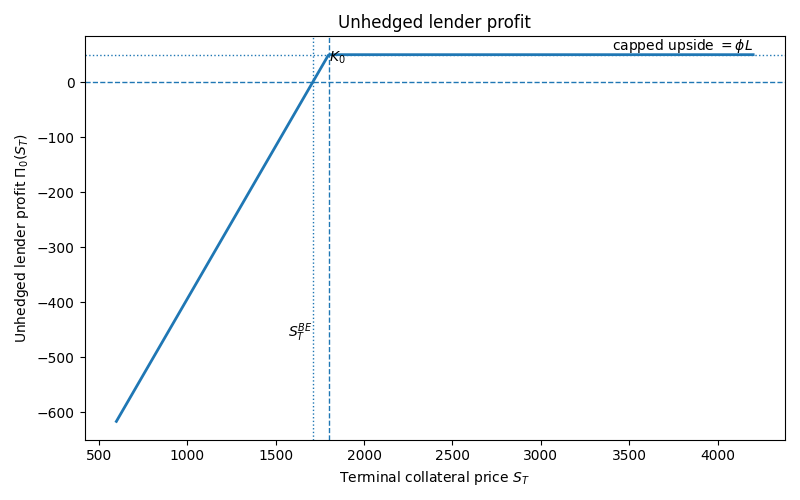
\includegraphics[width=1\linewidth]{Figure_1.png}
    \caption{Unhedged lender profit $\Pi_0(S_T)$ as a function of terminal collateral price $S_T$. The upper flat region equals $\phi L$, showing that the lender’s upside is capped by merchant fee revenue. The payoff begins to decline once $S_T < K_0$ and becomes negative when $S_T< S_T^{BE}$.}
    \vspace{-0.5em}
    \begin{flushleft}
    \footnotesize \textit{Source: Authors' own work.}
    \end{flushleft}
\end{figure}

From a financial-instrument perspective, the unhedged contract has a capped-upside and downside-exposed payoff. The lender’s maximum profit is fixed at $\phi L$, but the lender absorbs losses when the collateral price falls sufficiently far below the LTV-implied threshold. This shortfall term has a put-like structure: the lender is exposed to

$$
(L - qS_T)^+
$$

The purpose of option hedging, introduced in the next subsection, is to modify this shortfall exposure by adding downside protection that increases in value when the collateral price declines.

\subsection{Option-Hedged Lending Model}

Section 4.1 showed that the unhedged loan exposes the lender to the collateral shortfall

$$
(L - qS_T)^+
$$

Using the notation introduced earlier, and recalling that $L=qK_0$, this shortfall can be rewritten as

$$
(L - qS_T)^+ = q(K_0 - S_T)^+
$$

This representation makes the option-like structure of the contract explicit. The lender’s downside exposure is equivalent to being short a put-like payoff on the collateral asset with an effective strike given by the LTV-implied threshold $K_0$. This is precisely why the notation $K_0$ is useful: it identifies the price level at which the loan begins to experience a shortfall and highlights the natural connection between the unhedged contract and put-option protection.

A natural hedge for this exposure is therefore to purchase long put options on the collateral asset. Suppose that at origination the lender buys one put option per unit of posted collateral, with strike $K$, maturity $T$, and per-unit premium $P_t(K,T)$. The total hedge premium paid at time $t$ is then

$$
qP_t(K,T)
$$

and the terminal payoff of the hedge is

$$
q(K - S_T)^+
$$

Relative to the unhedged structure, the option hedge adds explicit downside protection that increases in value when the collateral price declines. The hedged lender profit can therefore be written as

$$
\Pi_H(S_T)=\phi L-qP_t(K,T)-q(K_0-S_T)^++q(K-S_T)^+.
$$

This expression has a straightforward interpretation. The lender still earns merchant fee revenue $\phi L$, but now pays an upfront insurance premium $qP_t(K,T)$. In exchange, the long put offsets part or all of the shortfall exposure from the unhedged contract. Section 5 will characterize the feasibility boundaries implied by this trade-off. At this stage, the focus is only on the structure of the hedge and the economic meaning of the strike choice.

The key design variable in the hedge is the put strike $K$. This strike determines the type of insurance policy the lender purchases. When

$$
K = K_0
$$

the option hedge matches the shortfall threshold of the loan exactly. In this case, once the collateral price enters the shortfall region, the long put offsets the lender’s shortfall dollar-for-dollar. Ignoring the premium cost, this is the natural benchmark case of an exact hedge.

When

$$
K < K_0
$$

the hedge is under-protective. The put only begins to pay off after the collateral price has already fallen below the shortfall threshold of the loan. As a result, part of the tail loss remains unhedged. For terminal prices below the option strike, $S_T \leq K$, the hedge pays off but does not fully eliminate the shortfall; the residual unprotected loss is $q(K_0-K)$. This case is economically attractive because lower-strike puts are generally cheaper, but the lender accepts residual downside risk.

When

$$
K > K_0
$$

the hedge is over-protective relative to the principal shortfall region. In this case, the put begins to pay off before the loan actually enters shortfall. This provides stronger protection, but it also requires paying a higher option premium. Therefore, the choice of $K$ determines how the lender trades off hedge cost against residual tail exposure.

This trade-off is central to the economics of the hedged contract. Smaller values of $K$ generally reduce the premium cost of protection, which improves upfront economics. At the same time, they leave more of the downside tail unprotected. Larger values of $K$ provide stronger insurance, but they make the hedge more expensive. The strike choice therefore acts as an insurance design variable: it determines how much risk is transferred to the options market and how much remains on the lender’s balance sheet.

The strike trade-off interacts closely with the choice of LTV. Since

$$
K_0 = \lambda S_t
$$

a lower LTV implies a lower effective strike $K_0$, pushing the shortfall region further into the downside tail. This makes the loan safer even before hedging. In the hedged setting, it also allows the lender to purchase lower-strike and therefore cheaper protection. From the lender’s perspective, lower $K_0$ is attractive for both risk and hedge-cost reasons. However, lower LTV also reduces borrower capital efficiency, because the borrower must post more collateral for the same loan amount. As in the unhedged case, practical market adoption discourages quoting excessively conservative LTV levels.

In practice, the hedge can be implemented using different option instruments. The most direct approach is to use options written on the same crypto asset that serves as collateral, whether through centralized venues or on-chain markets. Alternatively, the lender may hedge using options on a crypto ETF or another closely related instrument, with an assumed conversion factor linking the hedge notional to the collateral exposure. The latter approach may be operationally convenient, but it introduces basis risk because the hedge asset and the posted collateral are no longer identical.

A second practical dimension is the choice of option maturity. Ideally, the option maturity should match the loan maturity so that hedge protection is aligned with the collateral exposure. Since the lender controls the tenor of the quoted loan, this alignment can often be enforced or at least made approximate. If an exact maturity match is unavailable, one possibility is to use a longer-dated option and close, monetize, or exercise the position at loan maturity, depending on the contract’s exercise style. If the option is American-style, early exercise is available; otherwise the position may need to be unwound before expiry. A shorter-dated option is also possible, but in that case the lender becomes exposed after the hedge expires unless the position is rolled. These maturity choices involve operational and pricing trade-offs and are therefore left outside the current algebraic treatment.

Several implementation frictions are also worth noting. In practice, strikes are discrete, hedge quantities may not match the collateral exposure exactly, and option prices incorporate bid-ask spreads and execution costs. These frictions do not change the core logic of the hedge, but they affect the exact profitability and feasibility region of the lending structure. For this reason, the present section treats the option hedge in idealized form and leaves the precise feasibility boundaries to the next section.

Figure 2 illustrates the hedged payoff structure for different choices of the put strike relative to $K_0$. When $K=K_0$, the shortfall region is exactly offset apart from the premium cost. When $K<K_0$, the lender remains exposed to residual tail loss below the option strike. When $K>K_0$, the hedge begins to pay before the shortfall region, providing stronger but more expensive protection. These payoff shapes make clear that the option strike $K$ is not merely a market input; it is a product-design variable that determines the form and cost of insurance embedded in the loan.

\begin{figure}[H]
    \centering
    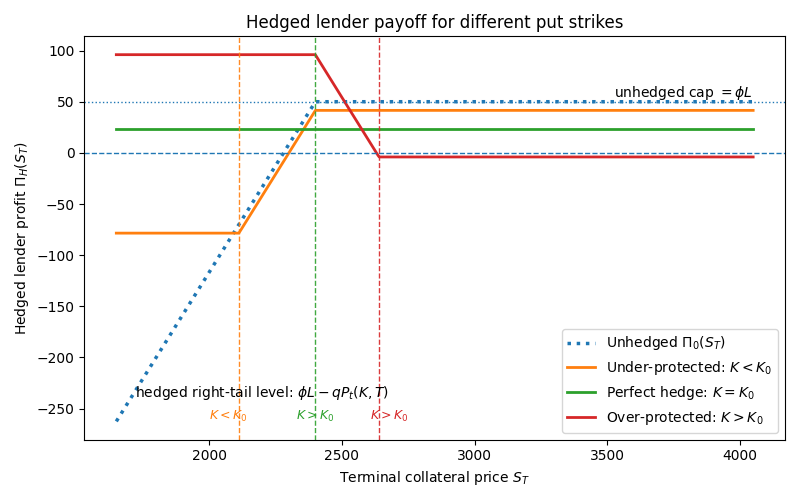
\includegraphics[width=1\linewidth]{Figure_2.png}
    \caption{Hedged lender profit $\Pi_H(S_T)$ for different choices of put strike $K$ relative to the LTV-implied threshold $K_0$. Lower strikes reduce hedge cost but leave more residual tail exposure, while higher strikes provide stronger protection at a higher premium.}
    \vspace{-0.5em}
    \begin{flushleft}
    \footnotesize \textit{Source: Authors' own work.}
    \end{flushleft}
\end{figure}


The option-hedged payoff therefore converts the lending problem into a trade-off between three quantities: fee revenue, hedge premium, and residual downside exposure. The strike $K$ determines how much of the collateral shortfall is transferred to the option market, while the LTV-implied threshold $K_0$ determines where the loan begins to experience shortfall in the first place. The next section turns this payoff structure into explicit market-observable algebraic feasibility bounds, deriving the conditions under which the hedge cost can be covered by fee revenue and the remaining downside exposure can be kept within an acceptable loss threshold.



\section{Algebraic Feasibility Bounds}

Section 4 introduced the hedged payoff

$$
\Pi_H(S_T)=\phi L-qP_t(K,T)-q(K_0-S_T)^++q(K-S_T)^+.
$$

This section derives algebraic conditions under which the hedged loan is economically feasible. The objective is to convert the payoff structure into simple bounds on the LTV-implied threshold $K_0$, given an observed option strike $K$, option premium $P_t(K,T)$, and merchant fee rate $\phi$.

Using the notation from Section 3, $P_t(K,T)$ denotes the option premium per unit of collateral, so the total hedge cost is $qP_t(K,T)$. Since $L=qK_0$, we can write

$$
q=\frac{L}{K_0}.
$$

This identity allows the feasibility conditions to be expressed directly in terms of $K_0$, the strike-like threshold that links the loan structure to the option market.

\subsection{Premium-Coverage Margin}

The relevant origination-time margin is the amount of fee revenue remaining after the hedge premium is paid:

$$
\text{PCM}(K_0,K,T) = 
\phi L - qP_t(K,T) = 
L\left( \phi -\frac{P_t(K,T)}{K_0} \right)
$$

This quantity measures whether the transaction can fund the hedge from its own fee revenue. It is not intended to capture speculative gains from the hedge in collateral drawdown states. In the exact and under-protective cases, $\text{PCM}$ is also the maximum terminal profit. In the over-protective case, terminal put payoffs may generate additional gains when the collateral price falls sharply, but those gains arise in adverse collateral states and are not the objective of the lending product. The framework therefore uses $\text{PCM}$ as the premium-coverage margin relevant for origination feasibility.

Non-negative premium coverage requires

$$
\text{PCM}(K_0, K,T) \geq 0
$$

Using the expression above and dividing by $L>0$,

$$
\phi- \frac{P_t(K,T)}{K_0} \geq 0
$$

which is equivalent to

$$
K_0 \geq \frac{P_t(K,T)}{\phi}
$$

This premium-coverage condition has a direct economic interpretation. The LTV-implied threshold must be large enough so that the collateral quantity $q=L/K_0$, and therefore the total hedge cost $qP_t(K,T)$, does not exceed the fee revenue $\phi L$.

\subsection{Worst-Case Profit for Under-Protection}

Now consider the case where the option strike is below or equal to the LTV-implied threshold:

$$
K \leq K_0
$$

This is the economically important case in which the lender uses an exact hedge $(K=K_0)$ or a cheaper under-protective hedge $(K<K_0)$. If $K<K_0$, the put option starts paying only after the loan has already entered the shortfall region. Therefore, the lender remains exposed to residual tail loss.

In deep downside states where $S_T\leq K$, the residual shortfall is capped by the gap between the loan’s effective strike $K_0$ and the option strike $K$. Per unit of collateral, this residual loss is $K_0 - K$. For $q$ units of collateral, the maximum residual loss is $q(K_0 - K)$.

The worst-case hedged profit is therefore

$$
\text{Profit}_{\min} = 
\phi L - qP_t(K,T) - q(K_0 - K)
$$

Substituting $q=L/K_0$,

$$
\text{Profit}_{\min} = 
\phi L - \frac{L}{K_0}P_t(K,T) - \frac{L}{K_0}(K_0 - K)
$$

A zero-loss feasibility condition requires

$$
\text{Profit}_{\min} \geq 0
$$

Thus,

$$
\phi L - \frac{L}{K_0}P_t(K,T) - \frac{L}{K_0}(K_0 - K) \geq 0
$$

Dividing by $L>0$,

$$
\phi - \frac{P_t(K,T)}{K_0} - \frac{(K_0 - K)}{K_0} \geq 0
$$

After re-arranging this becomes

$$
\frac{K - P_t(K,T)}{K_0} \geq 1 - \phi
$$

Assuming $0<\phi<1$, this implies

$$
K_0 \leq \frac{K - P_t(K,T)}{1 - \phi}
$$

This is the upper feasibility boundary for $K_0$. Economically, it says that $K_0$ cannot be too high relative to the selected option strike $K$. A higher $K_0$ corresponds to a higher LTV and a larger unprotected gap $K_0-K$, which increases residual tail loss.

\subsection{Worst-Case Profit under Over-Protection}

The previous subsection considered the exact-hedge and under-protective cases, where

$$
K \leq K_0.
$$

In this region, the option strike is at or below the loan’s LTV-implied shortfall threshold, so the lender may retain residual downside exposure equal to the gap between $K_0$ and $K$. We now consider the opposite case,

$$
K > K_0.
$$

This is the over-protective case. The put option begins paying before the collateral value falls below the loan principal. Equivalently, the option strike is above the loan’s shortfall threshold, so the hedge provides protection even in states where the collateral would still be sufficient to cover the loan.

Starting from the hedged payoff,

$$
\Pi_H(S_T)=\phi L-qP_t(K,T)-q(K_0-S_T)^++q(K-S_T)^+.
$$

consider the terminal hedge-shortfall component,

$$
-(K_0-S_T)^+ + (K-S_T)^+
$$

When $K>K_0$, this component is always non-negative. If $S_T\geq K$, both option-like terms are zero. If $K_0\leq S_T<K$, the loan has no collateral shortfall, but the put is already in the money. If $S_T<K_0$, the put payoff more than offsets the collateral shortfall. Therefore, the over-protective hedge does not leave residual terminal downside exposure.

As a result, the worst-case profit is not generated by a deep downside state. Instead, the lowest profit occurs when the put expires worthless and the lender has simply paid the hedge premium. Therefore,

$$
\text{Profit}_{\min} = \phi L - qP_t(K,T).
$$

Similarly to Section 5.2, the zero-loss condition is

$$
\text{Profit}_{\min} \geq 0
$$

or equivalently,

$$
K_0 \geq \frac{P_t(K,T)}{\phi}.
$$

Combining this with the over-protection condition $K_0<K$, the over-protective feasible region is

$$
K_0 \in \left[   \frac{P_t(K,T)}{\phi}, K \right).
$$

This result shows that over-protective structures are governed by a different feasibility condition than under-protective structures. In the under-protective case, feasibility must control both hedge premium and residual tail exposure. In the over-protective case, the terminal shortfall is fully covered, so feasibility reduces to whether merchant fee revenue can cover the hedge premium.

\subsection{Feasible Interval for $K_0$}

Combining the premium-coverage condition, the hedge-strike regime, and the worst-case loss condition gives the feasible set for the LTV-implied threshold $K_0$. Because the hedged payoff behaves differently depending on whether the option strike is below or above the loan’s shortfall threshold, it is useful to first write the feasible region branch by branch.

In the exact-hedge and under-protective case,

$$
K\leq K_0
$$

the feasible interval is

$$
K_0 \in \left[ 
\max\left(K, \frac{P_t(K,T)}{\phi} \right),
\frac{K - P_t(K,T)}{1 - \phi}
 \right].
$$

The left boundary combines two requirements: $K_0\geq K$, which keeps the structure in the exact-hedge or under-protective region, and $K_0\geq P_t(K,T)/\phi$, which ensures that fee revenue covers the hedge premium. The right boundary ensures that, in the under-protective region, the residual unprotected tail loss does not exceed the surplus left after paying for the hedge.

In the over-protective case,

$$
K > K_0
$$

the put option begins paying before the collateral value reaches the loan’s shortfall threshold. In this region, there is no residual terminal tail loss left by the hedge. Therefore, feasibility is governed by the premium-coverage condition together with the over-protection condition. The feasible region is

$$
K_0 \in \left[   \frac{P_t(K,T)}{\phi}, K \right).
$$

The general zero-loss feasible set is therefore the union of the over-protective and exact/under-protective branches:

$$
\left[   \frac{P_t(K,T)}{\phi}, K \right) \cup
\left[ 
\max\left(K, \frac{P_t(K,T)}{\phi} \right),
\frac{K - P_t(K,T)}{1 - \phi}
 \right].
$$

This union can be written as a single compact interval when the option quote is not too expensive relative to fee revenue. To see this, define

$$
a:=\frac{P_t(K,T)}{\phi}
$$

and

$$
b:=\frac{K-P_t(K,T)}{1-\phi}.
$$

The over-protective branch is $[a,K)$, while the exact/under-protective branch is $[\max(K,a),b]$. The union becomes one connected positive-width interval when the two branches connect through the boundary $K_0=K$. This requires

$$
a<K<b.
$$

The first inequality, $a<K$, is equivalent to

$$
P_t(K,T)<\phi K.
$$

The second inequality, $K<b$, is also equivalent to the same condition. Indeed,

$$
K<\frac{K-P_t(K,T)}{1-\phi}
$$

is equivalent, since $1-\phi>0$, to

$$
K(1-\phi)<K-P_t(K,T),
$$

which simplifies to

$$
P_t(K,T)<\phi K.
$$

Thus, when

$$
P_t(K,T)<\phi K,
$$

the over-protective branch covers

$$
\left[\frac{P_t(K,T)}{\phi},K\right),
$$

while the exact/under-protective branch begins at $K_0=K$ and extends to

$$
\frac{K-P_t(K,T)}{1-\phi}.
$$

The two branches therefore connect at $K_0=K$, and the global feasible set becomes

$$
K_0 \in
\left[
\frac{P_t(K,T)}{\phi},
\frac{K-P_t(K,T)}{1-\phi}
\right].
$$

This interval is the central algebraic feasibility result. It is not only the exact-hedge interval. Rather, it is the global zero-loss interval obtained by combining the over-protective, exact-hedge, and under-protective cases.

The same derivation gives a simple market-observable feasibility test:

$$
P_t(K,T)<\phi K,
$$

or equivalently,

$$
\frac{P_t(K,T)}{K}<\phi.
$$

Thus, before imposing the additional admissibility restriction $0<K_0<S_t$, an option quote passes the zero-loss feasibility screen if its premium-to-strike ratio is below the merchant fee rate. Quotes with $P_t(K,T)\ge \phi K$ are too expensive relative to fee revenue, while quotes with $P_t(K,T)<\phi K$ generate a positive-width zero-loss feasible set.

The interval remains necessary because the lender does not only need to know whether a feasible structure exists. The lender also needs to know which LTVs can be quoted. Once the lender observes the current spot price $S_t$, the merchant fee rate $\phi$, and the market option quote $(K,P_t(K,T))$, the feasible $K_0$ interval can be translated into an admissible LTV interval through

$$
K_0=\lambda S_t.
$$

Before imposing the admissibility restriction $0<K_0<S_t$, the raw LTV bounds are

$$
LTV_{\text{left}}
=
\frac{1}{S_t}\frac{P_t(K,T)}{\phi},
$$

and

$$
LTV_{\text{right}}
=
\frac{1}{S_t}\frac{K-P_t(K,T)}{1-\phi}.
$$

The feasible loan structures are then obtained by intersecting the $K_0$ interval with the economically admissible region

$$
0<K_0<S_t,
$$

or equivalently,

$$
0<\lambda<1.
$$

Thus, after imposing admissibility, the raw LTV interval is intersected with $(0,1)$, and the quote is usable only if the adjusted interval remains non-empty.

If the resulting LTV interval is empty, the option quote cannot support a zero-loss hedged loan under the model assumptions. If the interval is non-empty, every LTV inside the interval corresponds to a feasible loan structure. The width of the interval measures how much flexibility the lender has in choosing the loan-to-value ratio.

Importantly, the loan amount $L$ cancels out of the feasibility interval. The loan size determines the scale of the transaction, but the existence of a feasible structure depends on the fee rate, the collateral spot price, and the option market terms.

\subsection{Bounded-Loss Extension}

The zero-loss condition

$$
\text{Profit}_{\min} \geq 0
$$

is conservative. In practice, the lender may be willing to tolerate a limited worst-case residual tail loss after the hedge premium has already been covered by fee revenue. The loss budget is not used to finance the option premium and is not treated as additional revenue. Instead, it measures how much residual shortfall exposure the lender is willing to retain when the hedge is under-protective.

Let $B\geq 0$ denote this maximum acceptable residual tail loss, and define the loss budget as a fraction of the loan amount:

$$
\beta := \frac{B}{L}.
$$

Throughout this extension, the premium-coverage condition remains separate from the residual-loss condition. Therefore, any feasible structure must still satisfy

$$
\phi L - qP_t(K,T) \geq 0,
$$

or equivalently, using $q=L/K_0$,

$$
K_0 \geq \frac{P_t(K,T)}{\phi}.
$$

The loss budget affects the exact-hedge and under-protective region, where

$$
K \leq K_0.
$$

In this region, the lender may retain residual downside exposure equal to the gap between the loan's shortfall threshold $K_0$ and the option strike $K$. The bounded-loss condition becomes

$$
\text{Profit}_{\min} \geq -B.
$$

Using the expression for $\text{Profit}_{\min}$ in the under-protective region,

$$
\phi L
-
\frac{L}{K_0}P_t(K,T)
-
\frac{L}{K_0}(K_0-K)
\geq
-B.
$$

Dividing by $L$,

$$
\phi
-
\frac{P_t(K,T)}{K_0}
-
\frac{K_0-K}{K_0}
\geq
-\beta.
$$

Rearranging gives

$$
K_0
\leq
\frac{K-P_t(K,T)}{1-\phi-\beta},
$$

provided that

$$
1-\phi-\beta>0.
$$

Thus, allowing a bounded residual-loss budget relaxes the right boundary of the feasible interval. The general bounded-loss feasible interval becomes

$$
K_0
\in
\left[
\frac{P_t(K,T)}{\phi},
\frac{K-P_t(K,T)}{1-\phi-\beta}
\right],
$$

before imposing the admissibility restriction

$$
0<K_0<S_t.
$$

When $\beta=0$, this reduces to the zero-loss interval:

$$
K_0
\in
\left[
\frac{P_t(K,T)}{\phi},
\frac{K-P_t(K,T)}{1-\phi}
\right].
$$

The bounded-loss interval also implies a simple market-observable screening condition. A positive-width bounded-loss feasible interval exists when

$$
\frac{K-P_t(K,T)}{1-\phi-\beta}
>
\frac{P_t(K,T)}{\phi}.
$$

Since $1-\phi-\beta>0$, this is equivalent to

$$
\phi\left(K-P_t(K,T)\right)
>
P_t(K,T)(1-\phi-\beta).
$$

Expanding and cancelling the common term $-\phi P_t(K,T)$ gives

$$
\phi K > P_t(K,T)(1-\beta),
$$

or

$$
P_t(K,T)
<
\frac{\phi}{1-\beta}K.
$$

Equivalently,

$$
\frac{P_t(K,T)}{K}
<
\frac{\phi}{1-\beta}.
$$

This relaxed screening condition should not be interpreted as allowing the loss budget to subsidize the hedge premium. The lower boundary $P_t(K,T)/\phi$ is unchanged. The relaxation arises because a positive $\beta$ permits a larger residual under-protected gap $K_0-K$, which increases the admissible right boundary of the $K_0$ interval.

As $\beta$ increases, while $1-\phi-\beta>0$, the lender permits more residual downside exposure in the under-protective region. This expands the feasible $K_0$ interval and can make additional option quotes feasible. However, the lender must still have enough fee revenue to pay for the hedge premium.

The feasible LTV bounds under bounded-loss feasibility are obtained by dividing the $K_0$ interval by the spot price $S_t$. Before imposing admissibility,

$$
LTV_{\text{left}}
=
\frac{1}{S_t}
\frac{P_t(K,T)}{\phi},
$$

and

$$
LTV_{\text{right}}(\beta)
=
\frac{1}{S_t}
\frac{K-P_t(K,T)}{1-\phi-\beta}.
$$

The final admissible LTV interval is obtained by intersecting these raw bounds with $(0,1)$. Thus, the bounded-loss extension provides a direct way to incorporate residual tail-risk appetite into the algebraic framework while preserving the market-observable structure of the feasibility screen.

\subsection{Risk-Based Interpretation of the Loss Budget}

The bounded-loss extension treats $B$ as the maximum loss the lender is willing to tolerate from residual downside exposure after the premium-coverage condition has been imposed. In the algebraic framework above, $B$ can be chosen directly as a risk appetite parameter. For example, a lender may decide that the worst-case residual loss should not exceed a fixed percentage of the loan amount, $B=\beta L$.

A more risk-based interpretation is to connect $B$ to a tail-risk measure. If the terminal collateral price $S_T$ is modeled as a random variable, then the hedged profit

$$
\Pi_H(S_T) = 
\phi L -
qP_t(K,T) -
q(K_0-S_T)^+
+
q(K-S_T)^+
$$

also becomes a random variable. Defining losses as

$$
\mathcal{L}_H=\max(-\Pi_H(S_T),0),
$$

the lender may choose $B$ so that it covers a tail-risk measure such as

$$
B = \text{CVaR}_{\alpha}(\mathcal{L}_H).
$$

Equivalently, if $B$ is specified in advance, a risk-based feasibility condition would require

$$
\text{CVaR}_{\alpha}(\mathcal{L}_H) \leq B.
$$

This interpretation provides a bridge between the algebraic bounds and probabilistic risk management. The present paper keeps the main analysis focused on market-observable feasibility conditions derived from option prices. A full two-stage framework, in which the algebraic bounds are first used as a market screen and then candidate structures are evaluated under simulated or empirically estimated collateral-price distributions, is left for future work.



\section{Empirical Feasibility Analysis}

\subsection{Empirical Methodology}

This section evaluates whether the algebraic feasibility conditions derived above can be satisfied using real-world crypto option market data. The empirical analysis uses historical ETH option data from Deribit and historical ETH spot prices over the period from January 2021 to August 2025. The option dataset contains daily observations of listed ETH option contracts, including option type, strike, expiration date, close price, and number of trades. The spot dataset contains daily ETH closing prices over the same period. The two datasets are merged by quote date so that each option quote is matched with the contemporaneous ETH spot price, which is then used both to compute option moneyness and to convert ETH-denominated option prices into USD-denominated premiums.

The empirical analysis focuses on put options, since the lender’s unhedged exposure has a shortfall payoff that can be partially or fully offset by a long put position. The analysis keeps only put options and filters out invalid observations, including quotes with missing prices, nonpositive option premiums, nonpositive strike prices, nonpositive spot prices, or nonpositive time to maturity. For each remaining quote, the option premium is converted into USD terms by multiplying the option price, quoted in ETH terms, by the contemporaneous ETH spot price. This gives the per-unit premium $P_t(K,T)$ used in the feasibility formulas.

For each option quote, the following variables are constructed:

$$
S_t,\quad
K,\quad
P_t(K,T),\quad
T-t,\quad
\frac{K}{S_t},\quad
\frac{P_t(K,T)}{K}.
$$

Here, $S_t$ is the ETH spot price on the option quote date, $K$ is the put strike, $P_t(K,T)$ is the per-unit USD premium of the put, and $T-t$ is the option time to maturity in days. The premium ratio $P_t(K,T)/K$ is included as a market-cost diagnostic because the feasibility of the zero-loss interval depends directly on whether the option premium is small enough relative to the merchant fee revenue and strike.

The main empirical exercise applies the global zero-loss feasibility interval from Section 5 to every option quote. The screen includes over-protective, exact-hedge, and under-protective structures. In the over-protective region, $K>K_0$, the put begins paying before the loan enters collateral shortfall; in the exact and under-protective regions, $K\le K_0$, the hedge either matches or begins below the loan’s shortfall threshold. Combining these regimes gives a single market-observable feasible interval for $K_0$.

For a given merchant fee rate $\phi$, the lower and upper boundaries for the global zero-loss feasible interval are computed as

$$
K_{0,\text{left}}
=
\frac{P_t(K,T)}{\phi}.
$$

and

$$
K_{0,\text{right}}
=
\frac{K-P_t(K,T)}{1-\phi}
$$

The interval is then intersected with the economically admissible region $0<K_0<S_t$. This gives

$$
K_{0, \text{left, adj}} = \max(K_{0, \text{left}}, 0)
$$

and

$$
K_{0, \text{right, adj}} = \min(K_{0, \text{right}}, S_t)
$$

An option quote is classified as feasible if

$$
K_{0, \text{right, adj}} >
K_{0, \text{left, adj}}
$$

For feasible quotes, the corresponding LTV interval is obtained by dividing the $K_0$ boundaries by the spot price:

$$
LTV_{\text{left}} = 
\frac{K_{0, \text{left, adj}}}{S_t}
$$

$$
LTV_{\text{right}} = 
\frac{K_{0, \text{right, adj}}}{S_t}
$$

The width of this interval measures how much flexibility the lender has in selecting an economically feasible loan-to-value ratio.

The analysis is performed over a grid of merchant fee rates,

$$
\phi \in \{3\%, 5\%, 8\%, 10\% \}.
$$

These values are used to evaluate how sensitive feasibility is to the amount of fee revenue available to fund the option hedge. The zero-loss case is treated as the main benchmark, since it corresponds to the strictest version of the feasibility condition.

Because the motivating lending product is short-term BNPL-style credit, the empirical analysis focuses on target loan maturities of approximately two, three, four, and six months. Option quotes are assigned to maturity buckets using the following windows:

$$
2M: \text{60-65 days},\quad
3M: \text{90-95 days},\\
4M: \text{120-125 days},\quad
6M: \text{180-185 days},\\
$$

The windows are defined so that the option maturity is at least as long as the intended loan horizon, with a small allowance for slightly longer-dated options. This reflects the practical requirement that hedge protection should not expire before the loan resolves.

The empirical results are reported at both the quote level and the day level. Quote-level feasibility measures the fraction of individual option quotes that support a feasible zero-loss lending structure. Day-level feasibility measures whether at least one feasible option quote exists on a given date for a given fee and maturity bucket. The day-level measure is more directly related to product availability: a lending platform does not require every option quote to be feasible, but it does require at least one implementable hedge in the market on the origination date.

The section also studies time variation in feasible lending capacity. For each date and merchant fee, the analysis computes the number of feasible quotes, whether at least one feasible quote exists, the best feasible LTV upper bound, and the median width of feasible LTV intervals. These statistics show whether feasible structures are stable across market environments or concentrated in specific periods.

Finally, the empirical analysis selects the best available zero-loss structure on each date according to a lender-oriented rule. Among all feasible quotes on a given date and fee level, the selected structure maximizes the normalized premium-coverage margin,

$$
\frac{\text{PCM}}{L} = 
\phi - \frac{P_t(K,T)}{K_0}
$$

Since this expression is increasing in $K_0$, each feasible quote is evaluated at the upper end of its admissible interval, $K_{0,\text{right,adj}}$. The best-structure analysis is not intended to identify the most borrower-attractive loan. Instead, it identifies the feasible zero-loss structure that preserves the largest share of fee revenue after hedge cost.

As a robustness check, the section also considers the bounded-loss extension from Section 5.5. The zero-loss case $\beta=0$ remains the main benchmark, while small positive values of $\beta$ are used to test whether allowing limited worst-case residual loss materially changes the empirical feasibility results.

Overall, the empirical section tests whether the theoretical feasibility intervals are non-empty under observed option market prices, how feasibility varies with fee revenue and loan maturity, and whether the resulting LTV ranges are economically meaningful for a crypto-collateralized lending product. The analysis therefore translates the algebraic bounds into a market-based screening exercise using real ETH option quotes. The feasibility framework itself follows from the earlier derivation, where the lending decision is expressed directly in terms of the spot price, fee rate, option strike, option premium, and feasible $K_0$ interval.

\subsection{Feasibility by Merchant Fee and Loan Maturity}

This subsection reports the main feasibility results across merchant fee rates and target loan maturities. For each option quote, the zero-loss feasibility interval is computed and translated into feasible LTV bounds. Results are reported at two levels. The quote-level statistics measure the fraction of individual option quotes that support a feasible structure. The day-level statistics measure whether at least one feasible quote exists on a given date, which is closer to the practical product question of whether a loan could be issued on that day.

\subsubsection{Quote-level feasibility}

Table 1 reports quote-level feasibility by merchant fee and target maturity bucket. The results show a clear monotonic pattern: feasibility increases with the merchant fee and decreases with loan maturity. Shorter maturities are easier to support because shorter-dated put protection is generally cheaper. Longer maturities require more expensive hedge protection and therefore produce fewer feasible quotes and lower feasible LTV upper bounds. After incorporating the global feasible interval, the lower LTV bound is driven by premium coverage rather than by the option strike itself, so the more informative maturity comparison is the feasibility rate and the upper end of the feasible LTV interval.

\begin{table}[htbp]
\centering
\caption{Quote-level feasibility across maturity buckets and merchant fees}
\label{tab:quote_level_feasibility}
\small
\begin{adjustbox}{max width=\textwidth}
\begin{tabular}{llrrrrrr}
\toprule
Fee & Maturity bucket & Total quotes & Feasible quotes & Feasibility rate & Median LTV lower & Median LTV upper & Median LTV width \\
\midrule
3\%  & 2M, 60--65D   & 3,246 & 1,545 & 47.6\% & 23.3\% & 60.5\% & 32.4\% \\
3\%  & 3M, 90--95D   & 1,889 & 699   & 37.0\% & 23.3\% & 54.1\% & 24.2\% \\
3\%  & 4M, 120--125D & 1,087 & 352   & 32.4\% & 20.0\% & 47.2\% & 17.5\% \\
3\%  & 6M, 180--185D & 705   & 116   & 16.5\% & 20.0\% & 38.1\% & 15.8\% \\
5\%  & 2M, 60--65D   & 3,246 & 2,079 & 64.0\% & 21.0\% & 66.3\% & 38.1\% \\
5\%  & 3M, 90--95D   & 1,889 & 1,008 & 53.4\% & 23.0\% & 60.3\% & 30.5\% \\
5\%  & 4M, 120--125D & 1,087 & 524   & 48.2\% & 20.0\% & 51.2\% & 23.1\% \\
5\%  & 6M, 180--185D & 705   & 220   & 31.2\% & 26.0\% & 46.1\% & 17.8\% \\
8\%  & 2M, 60--65D   & 3,246 & 2,630 & 81.0\% & 20.0\% & 73.0\% & 44.8\% \\
8\%  & 3M, 90--95D   & 1,889 & 1,369 & 72.5\% & 23.1\% & 68.1\% & 36.1\% \\
8\%  & 4M, 120--125D & 1,087 & 708   & 65.1\% & 18.8\% & 58.4\% & 30.5\% \\
8\%  & 6M, 180--185D & 705   & 358   & 50.8\% & 28.8\% & 58.4\% & 23.0\% \\
10\% & 2M, 60--65D   & 3,246 & 2,914 & 89.8\% & 19.0\% & 77.2\% & 48.1\% \\
10\% & 3M, 90--95D   & 1,889 & 1,550 & 82.1\% & 23.3\% & 72.6\% & 40.1\% \\
10\% & 4M, 120--125D & 1,087 & 798   & 73.4\% & 18.0\% & 62.5\% & 32.0\% \\
10\% & 6M, 180--185D & 705   & 433   & 61.4\% & 27.5\% & 61.1\% & 26.9\% \\
\bottomrule
\end{tabular}
\end{adjustbox}
\vspace{-0.5em}
\begin{flushleft}
\footnotesize \textit{Source: Authors' own work.}
\end{flushleft}
\end{table}

Several observations follow from the table. First, at a 5\% merchant fee, approximately 64.0\% of 2M quotes are feasible, compared with only 31.2\% of 6M quotes. Second, the median feasible LTV upper bound also declines with maturity: at the same 5\% fee, the median upper bound is approximately 66.3\% for 2M loans but only 46.1\% for 6M loans. Thus, longer maturities are not only less frequently feasible; when they are feasible, they tend to require more conservative collateralization.

The fee effect is also strong. For 2M loans, quote-level feasibility rises from 47.6\% at a 3\% fee to 89.8\% at a 10\% fee. After incorporating the global feasible interval, which includes over-protective structures with $K_0<K$, the feasible LTV ranges become substantially wider. For 2M loans, the median feasible LTV width increases from approximately 32.4 percentage points at a 3\% fee to approximately 48.1 percentage points at a 10\% fee. This reflects the fact that lower-LTV, over-protective structures can be feasible as long as fee revenue covers the hedge premium. This suggests that higher merchant fees do not merely make feasibility more likely; they also give the lender more flexibility in choosing an admissible LTV inside the feasible interval.

The upper LTV bound should be interpreted as the most aggressive feasible LTV supported by a quote, while the lower bound is the minimum LTV required for fee revenue to cover the hedge premium. The interval width therefore measures the product-design flexibility available to the lender.

\subsubsection{Day-level feasibility}

Table 2 reports the same analysis at the day level. A day is classified as feasible if at least one option quote in the relevant fee and maturity bucket supports a zero-loss lending structure. This measure is more directly related to product availability, since a platform does not need every listed option quote to be feasible; it only needs at least one implementable hedge on the origination date.

The denominator in each maturity bucket is the number of dates on which at least one option quote is available in that maturity window, rather than the full number of calendar days in the sample.

\begin{table}[htbp]
\centering
\caption{Day-level feasibility across maturity buckets and merchant fees}
\label{tab:day_level_feasibility}
\small
\begin{adjustbox}{max width=\textwidth}
\begin{tabular}{llrrrrr}
\toprule
Fee & Maturity bucket & Total days & Feasible days & Day feasibility rate & Median feasible quotes per day & Median total quotes per day \\
\midrule
3\%  & 2M, 60--65D   & 336 & 308 & 91.7\%  & 4.0 & 9.0  \\
3\%  & 3M, 90--95D   & 232 & 184 & 79.3\%  & 2.0 & 8.0  \\
3\%  & 4M, 120--125D & 108 & 93  & 86.1\%  & 3.0 & 10.0 \\
3\%  & 6M, 180--185D & 107 & 62  & 57.9\%  & 1.0 & 6.0  \\
5\%  & 2M, 60--65D   & 336 & 333 & 99.1\%  & 6.0 & 9.0  \\
5\%  & 3M, 90--95D   & 232 & 208 & 89.7\%  & 4.0 & 8.0  \\
5\%  & 4M, 120--125D & 108 & 100 & 92.6\%  & 5.0 & 10.0 \\
5\%  & 6M, 180--185D & 107 & 80  & 74.8\%  & 1.0 & 6.0  \\
8\%  & 2M, 60--65D   & 336 & 335 & 99.7\%  & 8.0 & 9.0  \\
8\%  & 3M, 90--95D   & 232 & 221 & 95.3\%  & 5.0 & 8.0  \\
8\%  & 4M, 120--125D & 108 & 108 & 100.0\% & 6.0 & 10.0 \\
8\%  & 6M, 180--185D & 107 & 97  & 90.7\%  & 3.0 & 6.0  \\
10\% & 2M, 60--65D   & 336 & 336 & 100.0\% & 8.0 & 9.0  \\
10\% & 3M, 90--95D   & 232 & 224 & 96.6\%  & 7.0 & 8.0  \\
10\% & 4M, 120--125D & 108 & 108 & 100.0\% & 7.0 & 10.0 \\
10\% & 6M, 180--185D & 107 & 104 & 97.2\%  & 3.0 & 6.0  \\
\bottomrule
\end{tabular}
\end{adjustbox}
\vspace{-0.5em}
\begin{flushleft}
\footnotesize \textit{Source: Authors' own work.}
\end{flushleft}
\end{table}

The day-level results are substantially stronger than the quote-level results. At a 5\% merchant fee, for example, 2M structures are feasible on 99.1\% of observed days, and 3M and 4M structures are feasible on 89.7\% and 92.6\% of days, respectively. The 6M bucket remains the most restrictive: at a 5\% fee, it is feasible on 74.8\% of days, with a median of only one feasible quote per day. Overall, these results suggest that, conditional on having access to the option chain, feasible hedged structures are available on most quote-availability days, especially for two- to four-month maturities and for higher merchant fees.

This distinction between quote-level and day-level feasibility is important. The quote-level results show that many individual option quotes do not satisfy the zero-loss feasibility condition. However, the day-level results show that the option chain often contains at least one usable hedge. Therefore, the empirical evidence is more favorable when interpreted from a product-availability perspective rather than from the perspective of arbitrary individual option quotes.

\subsubsection{Fee sensitivity}

The fee sensitivity plot summarizes the effect of merchant fee revenue across all target maturities.

\begin{figure}[H]
    \centering
    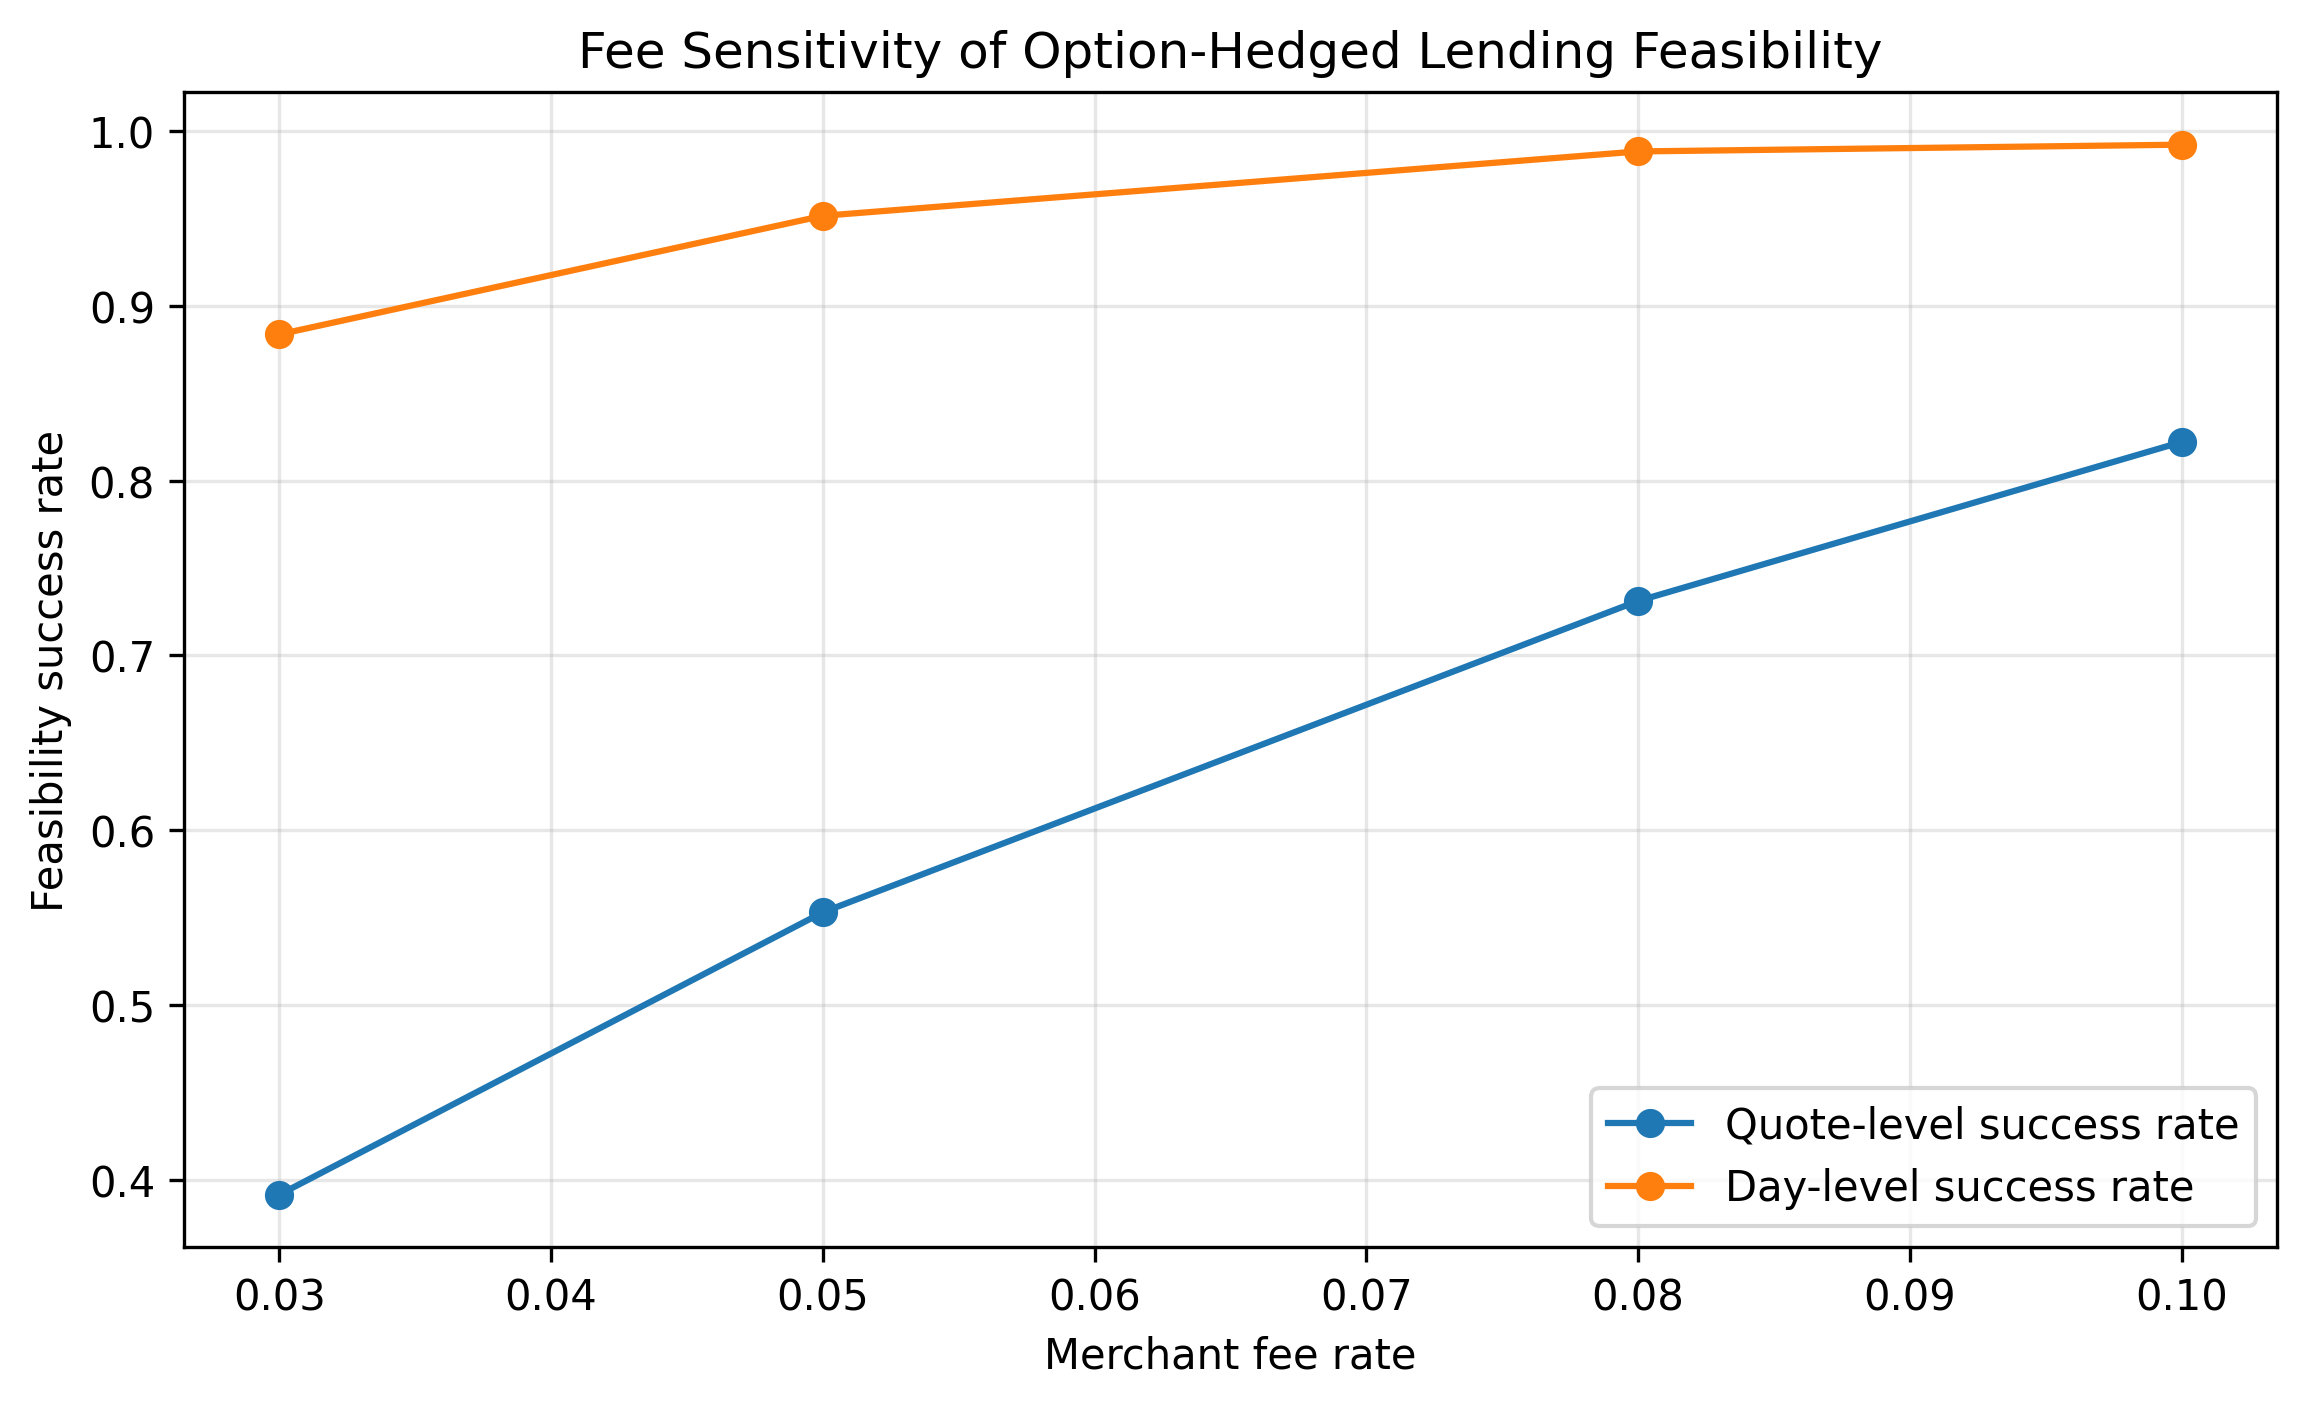
\includegraphics[width=1\linewidth]{image.png}
    \caption{Fee sensitivity of option-hedged lending feasibility. The figure reports quote-level and day-level feasibility success rates across merchant fee levels.}
    \vspace{-0.5em}
    \begin{flushleft}
    \footnotesize \textit{Source: Authors' own work.}
    \end{flushleft}
\end{figure}

Both increase with the merchant fee, but they do so in different ways. Quote-level feasibility increases strongly from roughly 39\% at a 3\% fee to roughly 82\% at a 10\% fee. Day-level feasibility is already high at a 3\% fee, at approximately 88\%, and rises to almost 99\% by the 8\%–10\% fee range.

The economic interpretation is that the merchant fee is a central driver of feasibility. Higher fee revenue makes it easier to cover the option premium and residual downside constraints, which increases the number of feasible option quotes and widens feasible LTV intervals. At the same time, the day-level curve shows that even lower fees can often support at least one feasible structure. Thus, the main role of higher fees is not only to make feasibility possible, but to increase market depth, flexibility, and reliability.

Under the global feasible interval, this widening is economically more substantial than in the under-protective-only screen, because the feasible set now includes conservative over-protective structures below the option strike.

Overall, these results suggest that option-hedged crypto-collateralized lending is most naturally supported for short and medium target maturities under moderate-to-high merchant fees. Two-, three-, and four-month structures are frequently feasible at the day level, while six-month structures remain the most restrictive and typically require either higher fee revenue or more conservative LTVs. The empirical results therefore support the model’s central prediction: feasibility is jointly determined by option prices, loan maturity, and fee revenue, rather than by collateralization alone.

\subsection{Time Variation and Best Available Zero-Loss Structures}

The previous subsection shows whether feasible structures exist across fee and maturity buckets. This subsection asks a slightly different question: conditional on feasibility, how attractive are the available structures over time? The analysis focuses on two objects. First, it tracks the best feasible LTV upper bound over time. Second, it selects the best available zero-loss structure on each date using the lender-oriented criterion

$$
\frac{\text{PCM}}{L} = \phi - 
\frac{P_t(K,T)}{K_0}
$$

For each feasible quote, this expression is evaluated at the upper end of the feasible interval, $K_{0,\text{right,adj}}$, since $\text{PCM}/L$ is increasing in $K_0$. Then, for each date and fee level, the quote with the highest $\text{PCM}/L$ is selected.

\subsubsection{Time variation in feasible LTV capacity}

\begin{figure}[H]
    \centering
    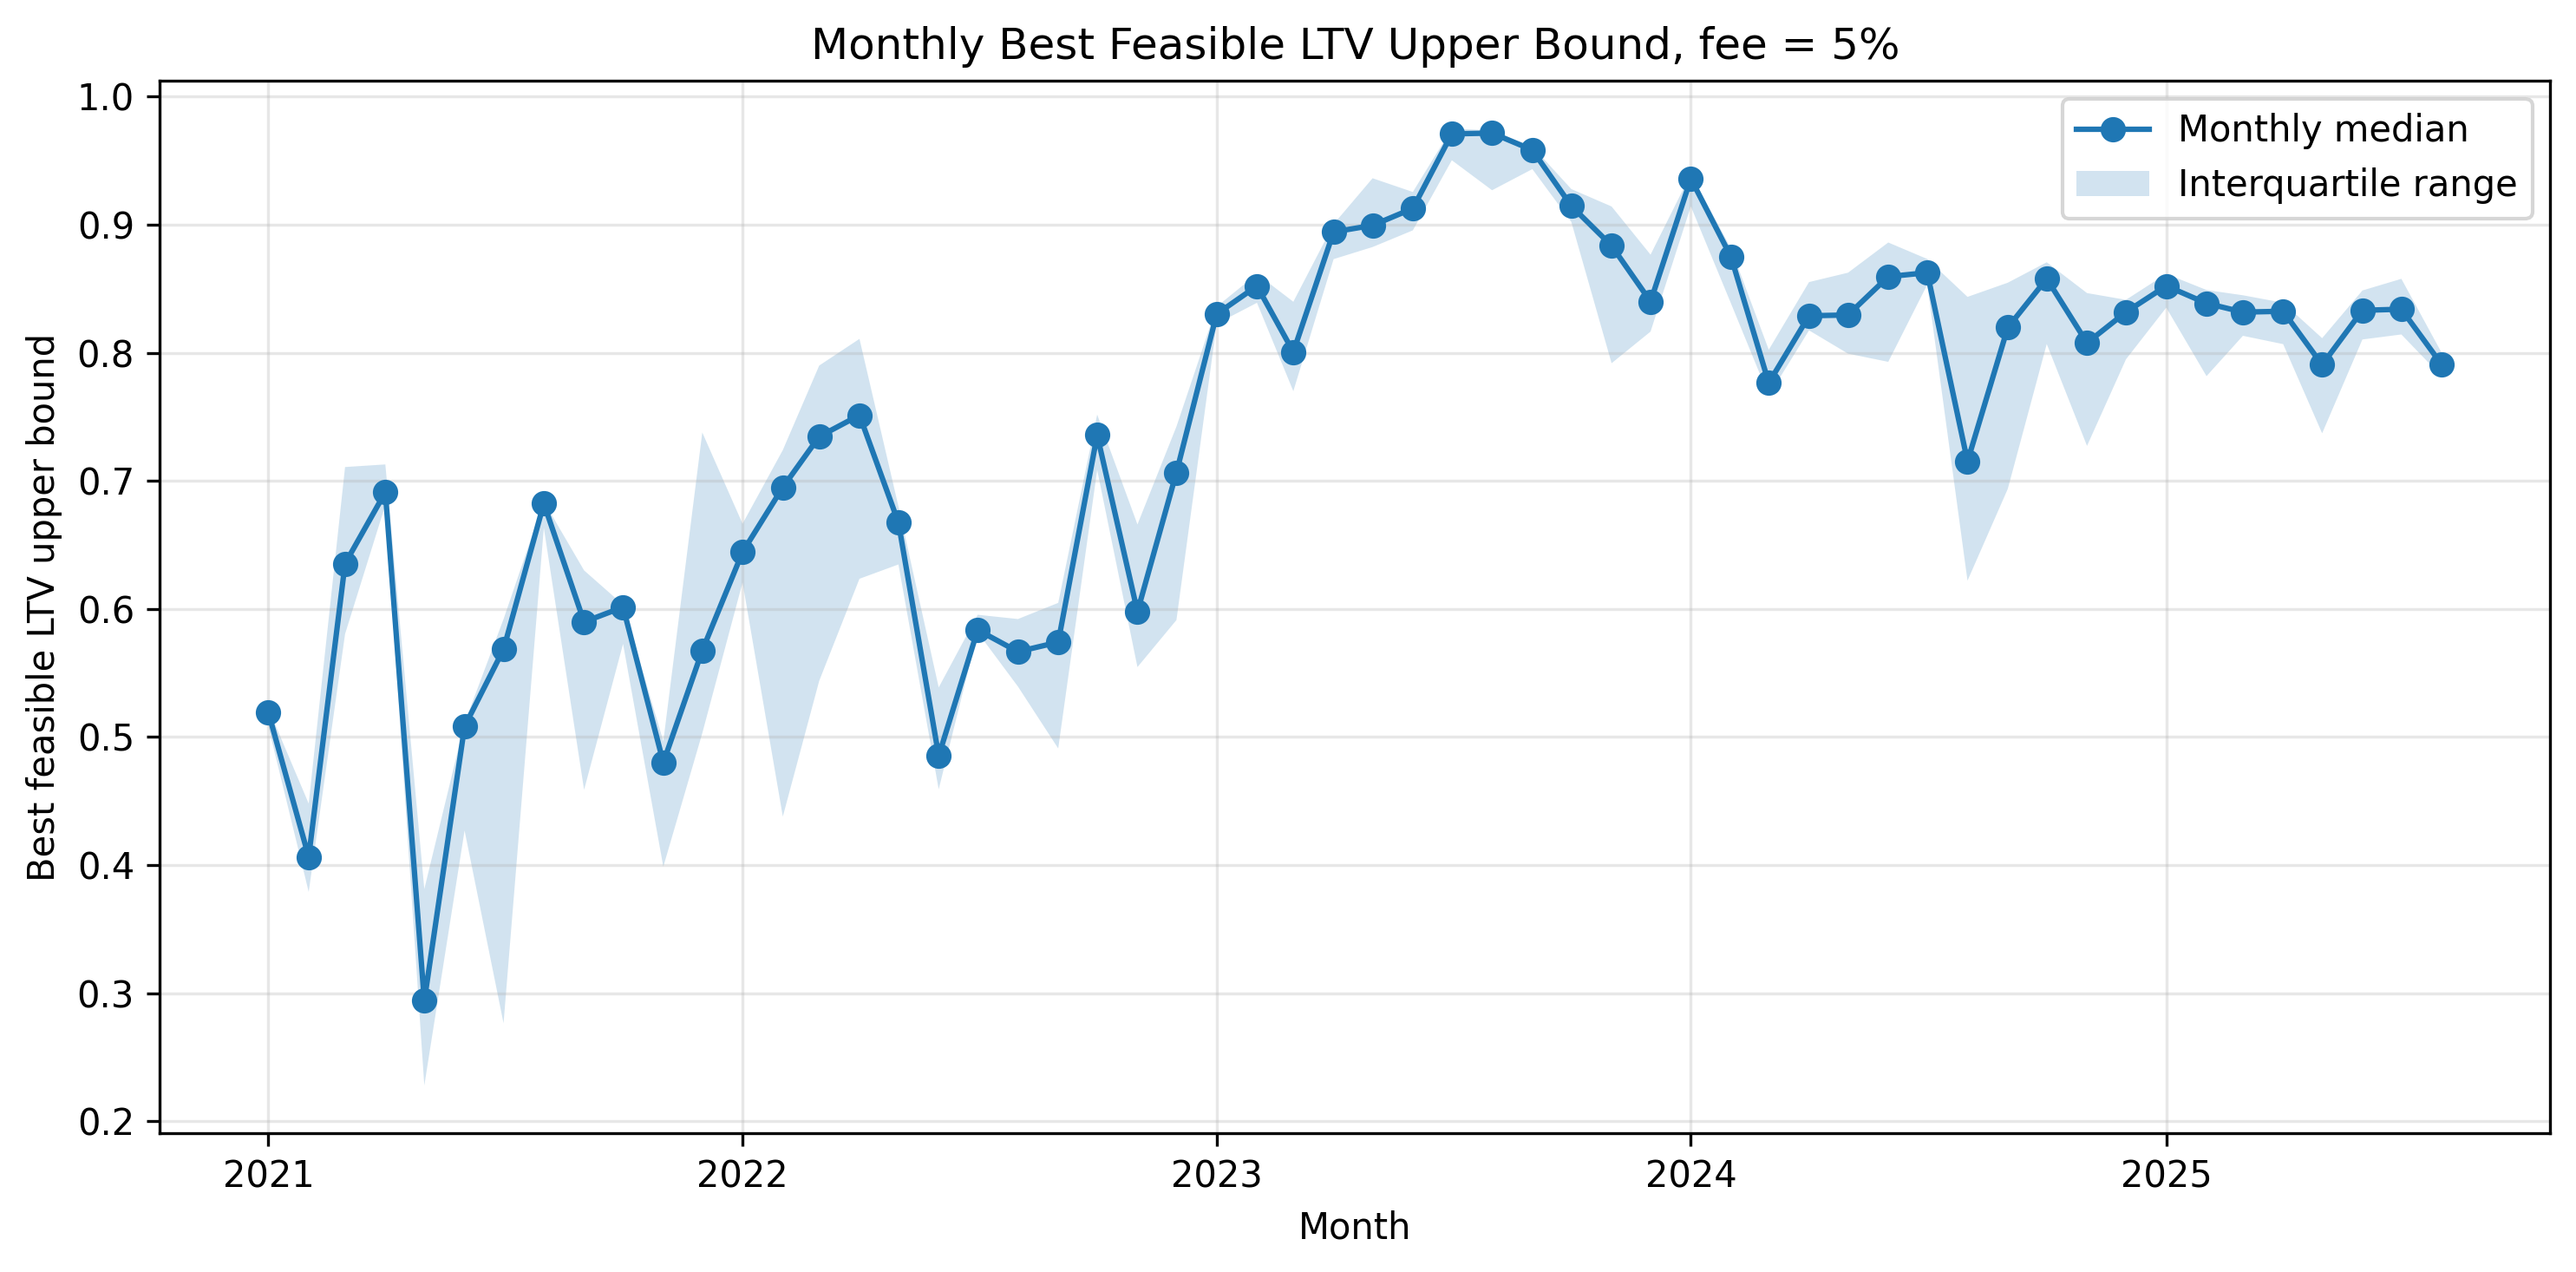
\includegraphics[width=1\linewidth]{image 1.png}
    \caption{Monthly best feasible LTV upper bound at a 5\% merchant fee. The line reports the monthly median of the best feasible LTV upper bound, while the shaded band reports the interquartile range across daily observations within each month.}
    \vspace{-0.5em}
    \begin{flushleft}
    \footnotesize \textit{Source: Authors' own work.}
    \end{flushleft}
\end{figure}

The figure shows that feasible LTV capacity is strongly time-varying. In the earlier part of the sample, especially during 2021 and parts of 2022, the monthly best feasible LTV upper bound is more volatile and often lies in the range of approximately 40\% to 70\%. This indicates that zero-loss structures may exist during these periods, but they often require relatively conservative collateralization.

Beginning around 2023, the best feasible LTV upper bound increases materially. The monthly median frequently rises into the 80\% to 95\% range, and the interquartile band becomes more stable. This suggests that, under the same 5\% merchant fee assumption, the option market more frequently supported higher-LTV zero-loss lending structures in the later part of the sample.

This result highlights an important practical implication of the framework. Feasibility is not a static property of the lending design. It depends on the market state, option prices, strike availability, and the relative cost of downside protection. Therefore, a platform using this framework would need to screen the option chain dynamically rather than rely on a fixed LTV schedule.

It is important to notice that the best feasible LTV upper bound and the PCM criterion answer different economic questions. The LTV-capacity measure asks how aggressive the loan could be while still satisfying the zero-loss feasibility constraint. The PCM criterion instead asks which feasible quote preserves the largest share of the merchant fee for the lender. These two criteria need not select the same option quote or the same LTV. In particular, maximizing PCM can favor cheaper, lower-strike hedges and therefore more conservative chosen LTVs, even when the option chain also supports higher feasible LTV upper bounds.

\subsubsection{Best available structure summary}

Table 3 reports the summary statistics for the best available zero-loss structure on each date and fee level. The selected structure maximizes $\text{PCM}/L$, so it should be interpreted as the most lender-attractive structure, not necessarily the most borrower-attractive one.

\begin{table}[htbp]
\centering
\caption{Best available feasible structure summary by merchant fee}
\label{tab:best_available_structures}
\small
\begin{adjustbox}{max width=\textwidth}
\begin{tabular}{lrrrrrrr}
\toprule
Fee & Days with best structure & Median PCM$/L$ & Mean PCM$/L$ & Median chosen LTV & Median LTV width & Median moneyness & Median TTM \\
\midrule
3\%  & 456 & 2.47\% & 2.16\% & 37.47\% & 25.48\% & 36.47\% & 65 \\
5\%  & 491 & 4.43\% & 3.96\% & 39.43\% & 29.31\% & 37.89\% & 65 \\
8\%  & 510 & 7.40\% & 6.81\% & 41.57\% & 33.33\% & 38.62\% & 65 \\
10\% & 512 & 9.41\% & 8.81\% & 42.81\% & 36.33\% & 38.81\% & 65 \\
\bottomrule
\end{tabular}
\end{adjustbox}
\vspace{-0.5em}
\begin{flushleft}
\footnotesize \textit{Source: Authors' own work.}
\end{flushleft}
\end{table}

The table shows that the best available structures retain most of the merchant fee after hedge cost. For example, at a 5\% fee, the median $\text{PCM}/L$ is approximately 4.43\%. At a 10\% fee, the corresponding value is approximately 9.41\%. This indicates that, conditional on finding a feasible quote, the hedge cost can be small relative to the fee revenue for the most lender-attractive structures.

However, after incorporating the global feasible interval, the median feasible LTV width around these best structures is much larger than in the under-protective-only screen, ranging from approximately 25.5 percentage points at a 3\% fee to 36.3 percentage points at a 10\% fee. Thus, the LTV selected by the PCM criterion is conservative, but the feasible interval around the selected quote can still support a broader range of lower-LTV structures.

This is not a weakness of the feasibility framework, but it clarifies the economic trade-off. If the lender selects structures by maximizing $\text{PCM}/L$ subject to zero-loss protection, the selected structure is likely to be conservative. More borrower-attractive structures with higher LTVs may still be feasible, but they would generally require selecting different option quotes or changing the selection criterion away from maximum PCM. This may require accepting lower $\text{PCM}/L$, higher hedge cost, or a less conservative loss constraint.

\subsubsection{Best available PCM over time}

\begin{figure}[H]
    \centering
    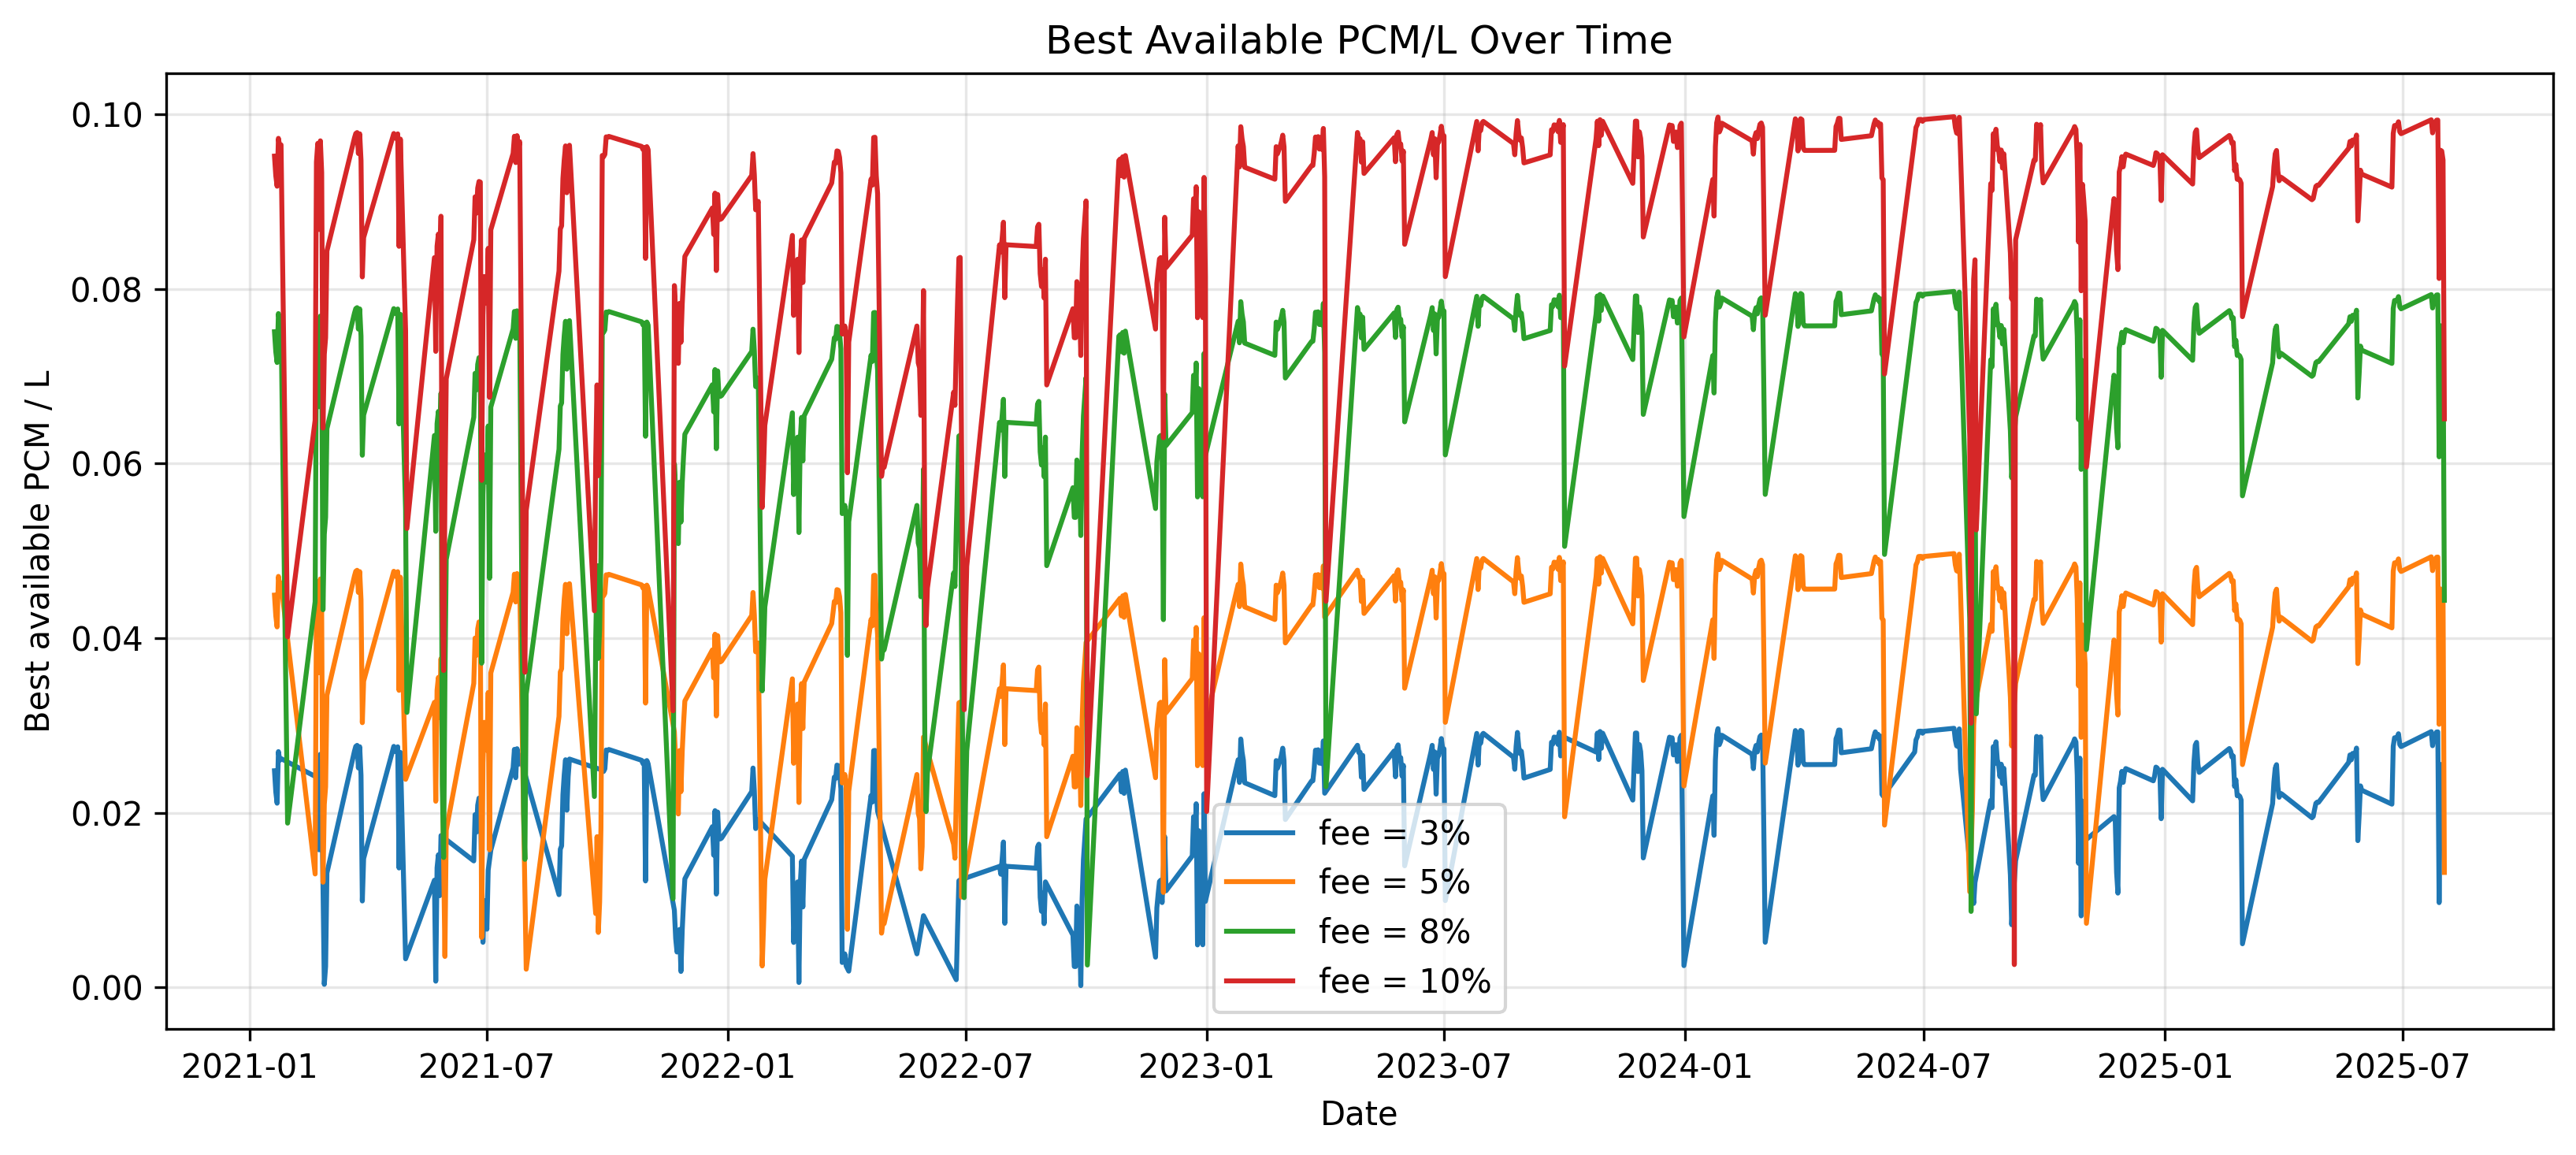
\includegraphics[width=1\linewidth]{image 2.png}
    \caption{Best available $\text{PCM}/L$ over time by merchant fee. For each date and fee level, the figure plots the highest normalized premium-coverage margin, $\text{PCM}/L$, among feasible zero-loss structures.}
    \vspace{-0.5em}
    \begin{flushleft}
    \footnotesize \textit{Source: Authors' own work.}
    \end{flushleft}
\end{figure}


The daily series is noisy because the selected structure depends on the available option chain, strike grid, traded quotes, and option premiums on each date. Nevertheless, the fee ordering is clear. Higher merchant fees consistently produce higher best available $\text{PCM}/L$.

The plot also shows that the best available $\text{PCM}/L$ can often remain close to the merchant fee level. For example, at $\phi=10\%$, the best daily $\text{PCM}/L$ frequently lies near 9\% to 10\%. At $\phi=5\%$, it often lies near 4\% to 5\%. This is consistent with Table 3 and suggests that, when the optimizer can select the most lender-attractive feasible quote, hedge costs can be relatively small compared with fee revenue.

At the same time, the sharp drops in the time series show that the best structure is not always stable. On some dates, the available option chain supports much less attractive economics. This reinforces the earlier point that the lending product should be evaluated through a dynamic market screen. A fixed product rule may fail to capture changes in option-market conditions.

Overall, the best-structure analysis adds an important qualification to the feasibility results. The option market frequently contains feasible zero-loss structures, and the structures with the highest $\text{PCM}/L$ can preserve most of the merchant fee. However, these structures tend to be short-dated and conservative in LTV. Therefore, the empirical findings support the economic feasibility of option-hedged lending, but also show that feasibility is strongest when the lender is willing to quote conservative LTVs or when fee revenue is sufficiently high.

\subsection{Bounded-Loss Robustness}

The previous results use the zero-loss benchmark, where the lender requires the hedged structure to have non-negative worst-case profit. This subsection relaxes that condition and allows the lender to tolerate a bounded residual loss. Specifically, the lender is allowed to lose at most a fraction $\beta$ of the loan amount in the worst-case residual exposure, so the loss budget is

$$
B = \beta L
$$

Under this extension, the right boundary of the feasible interval becomes

$$
K_{0,\text{right}}(\beta)
=
\frac{K-P_t(K,T)}{1-\phi-\beta},
$$

subject to

$$
1 - \phi - \beta > 0
$$

The parameter $\beta$ is therefore interpreted as a residual tail-loss budget, not as additional fee revenue used to pay for the option premium. Accordingly, the premium-coverage lower boundary remains unchanged, while $\beta$ only relaxes the residual tail-loss boundary.

The zero-loss benchmark corresponds to $\beta=0$. The empirical analysis compares day-level feasibility rates for

$$
\beta \in \{0\%, 1\%, 3\%, 5\% \}.
$$

Day-level feasibility is used because it is the most relevant product-availability measure: it asks whether at least one feasible hedged structure exists on a given date.

\begin{figure}[H]
    \centering
    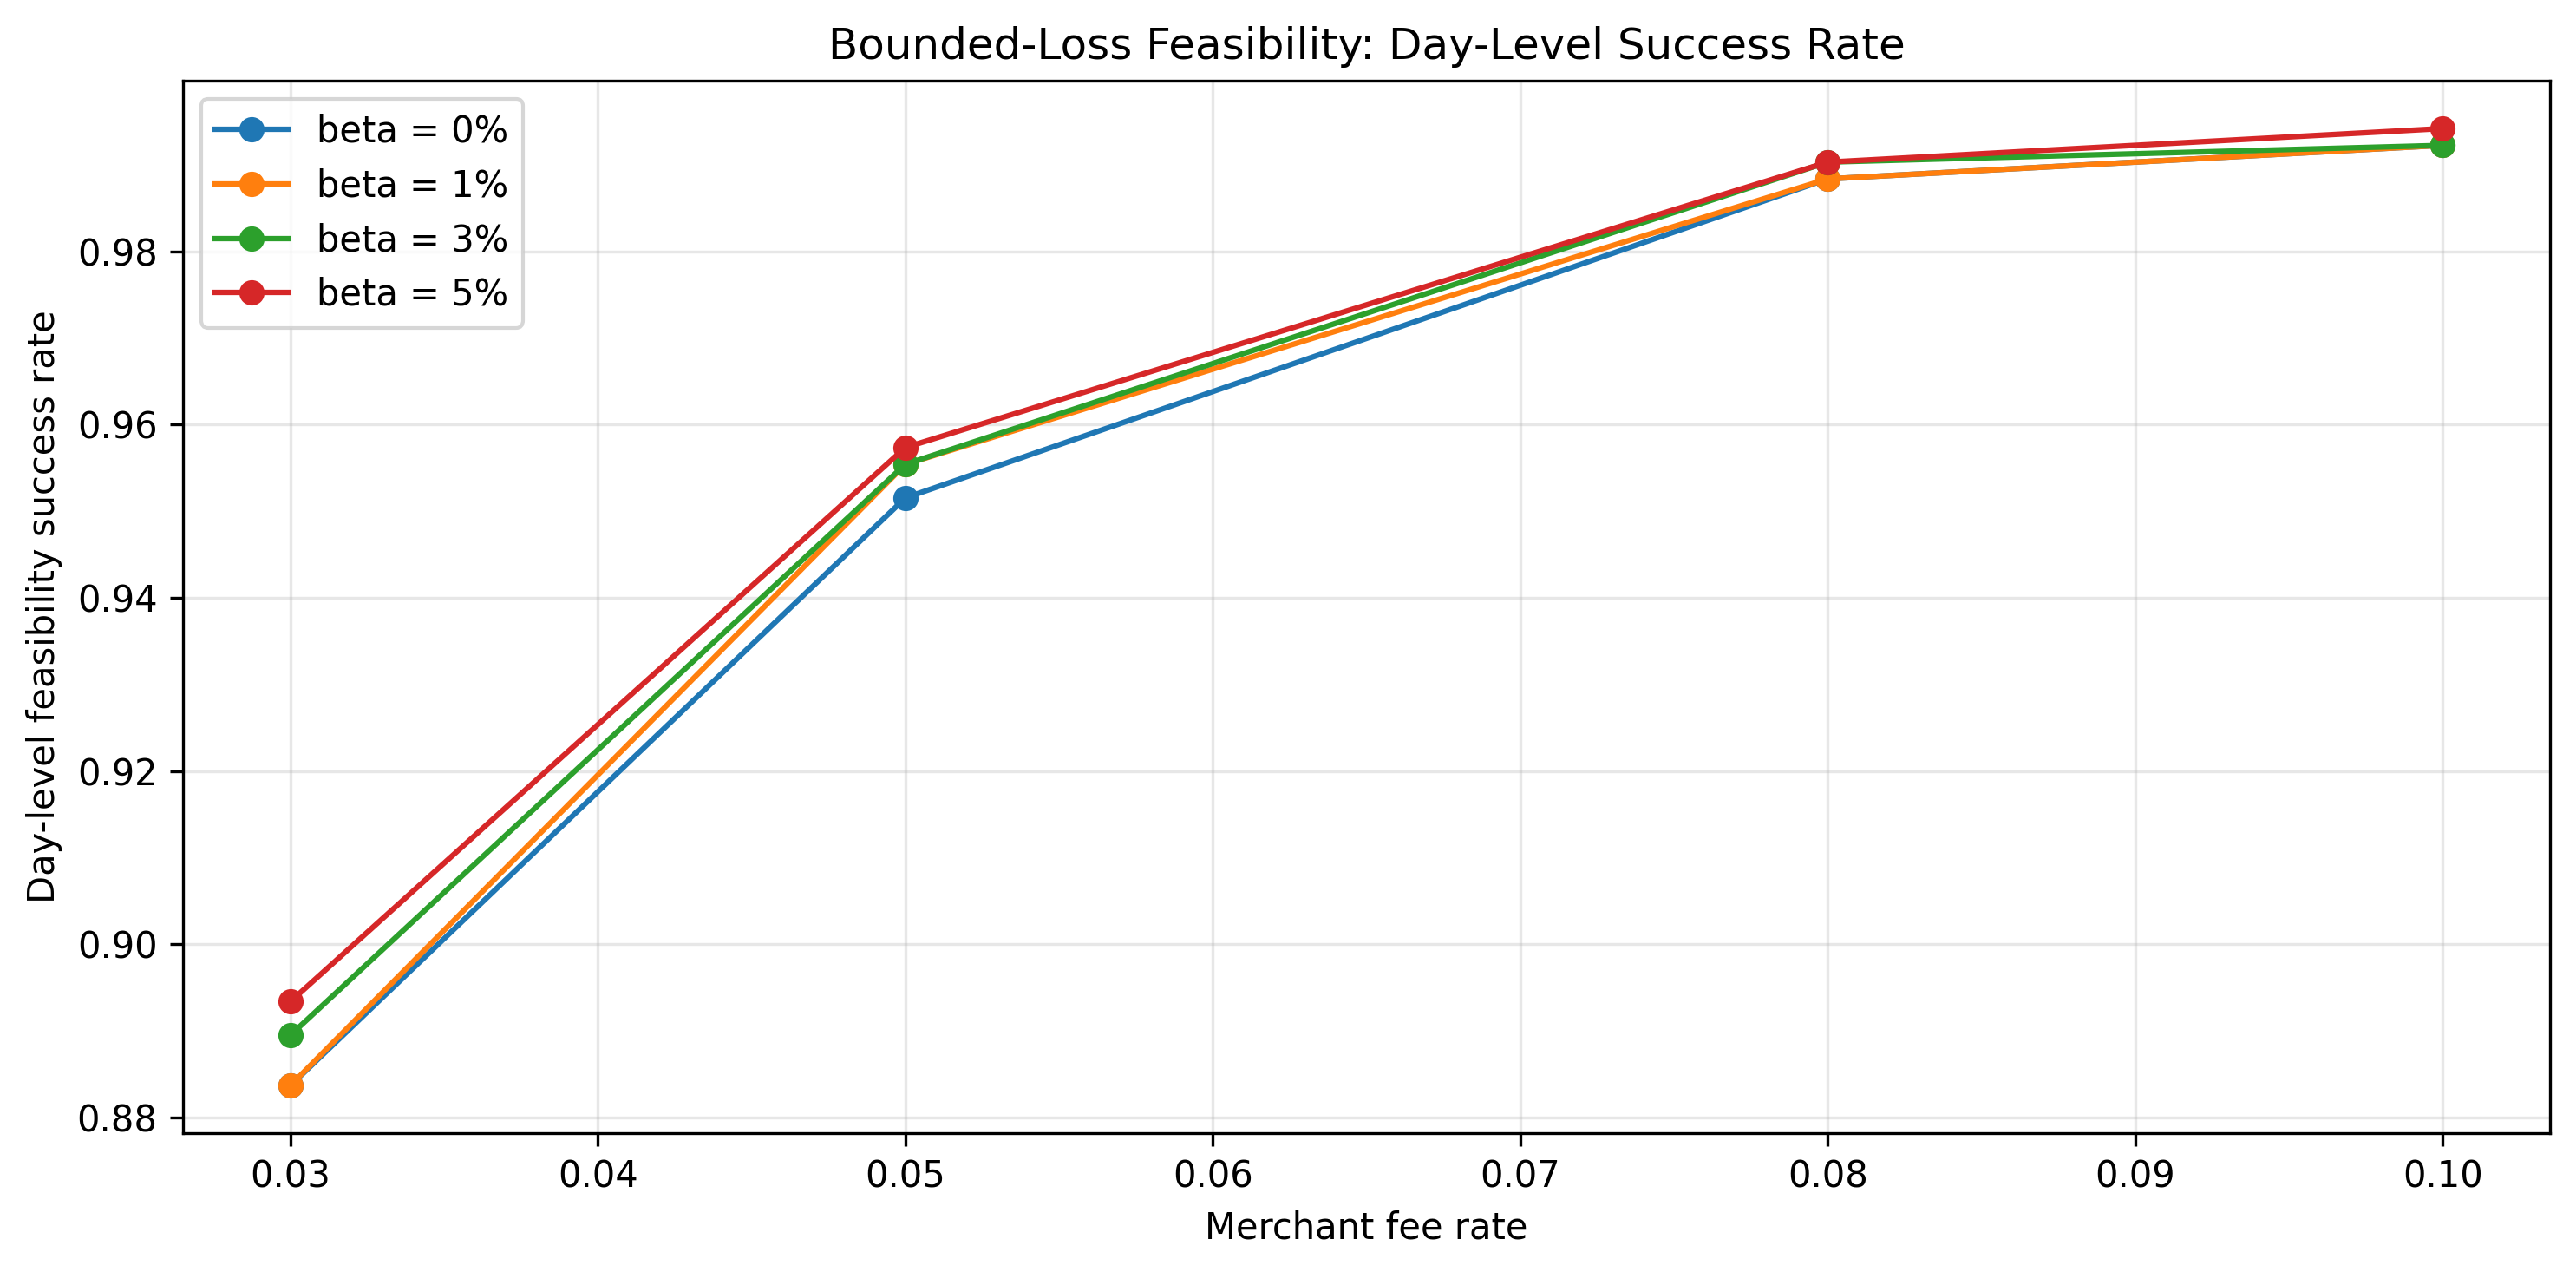
\includegraphics[width=1\linewidth]{image 3.png}
    \caption{Day-level feasibility under bounded-loss budgets. The figure reports day-level success rates for $\beta \in \{0\%,1\%,3\%,5\%\}$ across merchant fee levels.}
    \vspace{-0.5em}
    \begin{flushleft}
    \footnotesize \textit{Source: Authors' own work.}
    \end{flushleft}
\end{figure}

Allowing a bounded loss budget increases day-level feasibility, but the effect is modest. At a 3\% merchant fee, the day-level feasibility rate increases from approximately 88.4\% under the zero-loss benchmark to approximately 89.3\% when $\beta=5\%$. At a 5\% merchant fee, the corresponding increase is from approximately 95.2\% to 95.7\%. For higher merchant fees, the curves are nearly saturated: at $\phi=8\%$ and $\phi=10\%$, day-level feasibility is already close to 99\%, so the additional effect of $\beta$ is small.

The economic interpretation is that the bounded-loss extension expands the feasible interval, but it does not fundamentally change the main empirical conclusion. Merchant fee revenue remains the dominant driver of day-level feasibility. Once the fee is high enough, the option chain already contains feasible zero-loss structures on most days, leaving little room for bounded-loss tolerance to improve the binary availability measure.

This result is useful as a robustness check. It shows that the zero-loss benchmark is not excessively restrictive at the day level. The main empirical finding is that feasible option-hedged lending structures frequently exist under observed ETH option prices, especially at moderate-to-high fees, and this conclusion does not depend on allowing residual worst-case losses. Instead, allowing positive $\beta$ mainly provides incremental flexibility and may increase the number of feasible quotes available to the lender, even if it has only a small effect on whether at least one feasible quote exists on a given day.

Overall, the bounded-loss analysis supports the interpretation of the zero-loss case as a conservative but informative benchmark. Relaxing the worst-case loss constraint slightly improves feasibility, particularly at lower fee levels, but the central product economics are still governed primarily by the merchant fee, loan maturity, and market price of downside protection.


\section{Discussion}

The framework developed in this paper should be interpreted as an origination-time feasibility analysis for a BNPL-like collateralized lending structure. At origination, the platform fixes the financed amount, collateral requirement, maturity, fee income, and hedge design. Within this setup, the derived feasibility interval identifies the set of loan structures for which the economics of the transaction can support the desired downside protection. The interval is therefore not only an algebraic object. It directly answers a practical risk-management question: which combinations of LTV, hedge strike, option premium, and fee revenue are compatible with a bounded-loss lending product?

The empirical results show that the feasibility interval can be used as a market-implied origination screen. Rather than selecting a fixed LTV or hedge strike independently of market conditions, the lender can use observed option prices to determine which lending structures are feasible at a given point in time. This is especially important for volatile collateral assets, where the cost of downside protection changes substantially across market regimes. In this sense, feasibility is not a static property of the product design. It depends jointly on collateral prices, available option strikes, option premia, maturity, and platform fee income.

The empirical findings also clarify the economic role of the merchant fee. Higher fee revenue expands the feasible region because it increases the amount of hedge cost that can be absorbed by the transaction. Shorter maturities are generally easier to support because shorter-dated downside protection is typically less expensive than longer-dated protection. The distinction between quote-level and day-level feasibility is also important. Many individual option quotes may fail the zero-loss screen, but the option chain can still contain at least one feasible hedge on a given origination date. From a product-availability perspective, the relevant question is therefore not whether every quote is feasible, but whether the market provides at least one implementable structure.

Although the empirical section uses crypto collateral, the framework itself is not crypto-specific. The same algebra applies to any collateral asset for which a protective option or comparable downside hedge is available. Crypto provides a demanding test case because of its high volatility, jump risk, and heavy-tailed return behavior. For assets with lighter tails and more stable price dynamics, the same feasibility logic may produce wider or more stable feasible regions, all else equal. However, this is ultimately an empirical question because feasibility also depends on hedge-market liquidity, implied volatility, strike availability, bid-ask spreads, and execution costs. Therefore, the empirical results should be interpreted as evidence from a demanding collateral setting rather than as a universal calibration across collateral classes.

Several limitations remain. First, the empirical implementation uses observed option prices, while actual hedge implementation may involve bid-ask spreads, limited order-book depth, execution slippage, transaction fees, and timing mismatch between loan origination and hedge execution. These frictions may reduce the practical size of the feasible interval, especially during periods of market stress when option liquidity deteriorates and downside protection becomes more expensive. The empirical analysis should therefore be viewed as a market-screening exercise rather than a fully execution-adjusted trading or lending backtest.

Second, the analysis abstracts from several product-design and implementation issues specific to BNPL-style lending. These include borrower demand, merchant adoption, custody arrangements, regulatory treatment, operational servicing, and borrower behavior after origination. These issues matter for commercial implementation, but they are separate from the feasibility question studied here: whether merchant fee revenue and observed option prices can support bounded-loss origination under the stated contract structure.

A further conceptual limitation is that the framework uses observed option prices, which reflect risk-neutral valuation. In a risk-neutral framework, the expected drift of the collateral asset is replaced by the risk-free rate, while the option surface reflects the market-implied distribution of future spot prices. The feasibility interval derived in this paper is therefore market-implied: it determines whether the platform can afford downside protection at currently observed option prices. However, the platform’s real-world profitability depends on the physical distribution of collateral returns, which may differ from the risk-neutral distribution because of risk premia, market cycles, and regime-dependent dynamics. This distinction is especially relevant for crypto collateral, where directional views and cyclicality can materially affect expected returns.

These limitations suggest several natural extensions. First, future work could incorporate execution-aware option prices by using bid-ask spreads, order-book depth, transaction fees, and realistic hedge execution rules. This would make it possible to measure how much of the theoretical feasible interval remains after implementation costs. Second, the same framework could be tested across different collateral assets, including liquid equities, equity indices, ETFs, or diversified collateral portfolios. This would help determine whether feasibility regions become wider or more stable for collateral classes with different volatility, liquidity, and tail-risk characteristics.

Future work could also combine the market-implied feasibility screen with estimates of the physical return distribution. This would allow candidate structures to be evaluated not only by whether they can be hedged at observed option prices, but also by expected profitability and tail risk under the platform’s real-world view of collateral dynamics. In this direction, the bounded-loss framework developed in the paper could be complemented with probabilistic criteria such as Value-at-Risk or Conditional Value-at-Risk, allowing comparison between fully protected structures and partially protected structures that may offer better economic efficiency while still satisfying a chosen risk tolerance.

A further extension would be to compare the option-hedged feasibility framework with carefully designed unhedged collateral policies. Such a comparison should not rely on an arbitrary fixed LTV, but instead should benchmark against unhedged LTV rules calibrated to a common risk objective, such as a target shortfall probability, historical drawdown tolerance, Value-at-Risk, Conditional Value-at-Risk, or a specified stress scenario. This would shift the analysis from feasibility to relative efficiency: future work could examine whether option-hedged structures allow higher borrowing capacity, lower residual losses, or more stable performance during collateral drawdowns than unprotected overcollateralized loans with comparable risk targets.

Overall, the framework should be viewed as a feasibility layer rather than a complete commercial lending model. It does not replace borrower underwriting, collateral policy, liquidation rules, execution controls, or portfolio-level risk management. Instead, it provides a transparent way to connect product economics with observed hedge prices. By converting collateral downside risk into an explicit market-implied cost, the model identifies when option-hedged collateralized lending can be originated under a specified loss constraint and when the market price of protection makes the structure economically unattractive.


\section{Conclusion}

This paper developed an algebraic framework for evaluating option-hedged BNPL-style collateralized lending, with crypto collateral serving as the motivating empirical setting. The central research question is whether a lender can originate a collateralized BNPL-like loan while keeping downside losses bounded, given the loan amount, collateral value, maturity, merchant fee revenue, and observed option-market prices.

The paper shows that this question can be reduced to market-observable feasibility bounds. For a given put option strike, premium, maturity, and merchant fee rate, the model identifies the interval of LTV-implied collateral thresholds that can support zero-loss or bounded-loss lending. Equivalently, the framework converts observed option quotes into feasible LTV ranges. A quote is economically useful only if fee revenue can cover the hedge premium and any residual downside exposure remains within the specified loss constraint.

The derived feasible interval provides a direct screening rule for loan origination. Higher merchant fee revenue expands the feasible region, while more aggressive LTVs and longer maturities make feasibility harder to achieve. Lower hedge strikes can reduce option premia but leave more residual downside exposure, while higher strikes provide stronger protection at greater cost. The model therefore turns collateralized loan design into a trade-off between borrower capital efficiency, hedge affordability, and lender downside protection.

Applying the framework to historical ETH put option data shows that feasibility is strongly increasing in merchant fee revenue and decreasing in loan maturity. Shorter-maturity structures are more frequently feasible and support wider feasible LTV intervals, while longer-maturity structures generally require either higher fee revenue or more conservative collateralization. The results also show that day-level feasibility is substantially stronger than quote-level feasibility: even when many individual option quotes are infeasible, the option chain often contains at least one implementable hedge on a given origination date.

The bounded-loss extension modestly increases feasibility, especially at lower fee levels, but does not change the central empirical conclusion. Product viability is governed primarily by merchant fee revenue, loan maturity, and the market price of downside protection. The main value of the framework is that it separates collateralization from hedge affordability: a loan is not feasible merely because it is overcollateralized, but because the remaining downside exposure can be protected at a market price consistent with the product’s revenue model.

Overall, the paper shows that option hedging can convert collateral downside risk into an explicit market-implied origination screen, but only when the cost of protection is compatible with the economics of the lending product. The framework is not a complete commercial lending model; rather, it provides a feasibility layer that can be extended with execution-aware hedge prices, broader collateral classes, and probabilistic risk criteria under real-world asset dynamics.


\bibliographystyle{apalike}
\bibliography{references}

\end{document}